\chapter{Basic Domain Theory in HOLCF}
\label{ch:holcf}

%%%%%%%%%%%%%%%%%%%%%%%%%%%%%%%%%%%%%%%%%%%%%%%%%%%%%%%%%%%%%%%%%%%%%%

\section{Introduction}

Isabelle/HOLCF is a library of domain theory, formalized within the logic of Isabelle/HOL. It is specifically intended to support denotational-style reasoning about recursive functional programs. It is specifically \emph{not} about doing abstract mathematics for its own sake; HOLCF only includes those parts of domain theory that are useful for reasoning about computation.

As was described in the first chapter, HOLCF has undergone various revisions during its history: The original version (\HOLCF{95}) was created by Regensburger \cite{regensburger94thesis, regensburger95holcf} as a way to reason about the LCF logic \cite{paulson87lcf} within Isabelle/HOL. The version from a few years later (\HOLCF{99}) was the next important milestone, representing the work of several contributors \cite{hol+lcf}. \HOLCF{99} offered improvements to the ``core'' of HOLCF---i.e., the parts that implemented the basic LCF functionality---and also introduced completely new functionality with the \textsc{Domain} package. The most recent version (\HOLCF{11}) includes many new improvements and extensions by the present author, covering both the LCF core and the various definition packages. This chapter will describe the new implementation of the core parts of \HOLCF{11}.

\paragraph{Contributions.} Although much of the core of \HOLCF{11} is quite similar to \HOLCF{99}, there are some significant recent improvements as well. The primary original contributions described in this chapter are mostly concerned with proof automation:
\begin{itemize*}
\item Using \emph{compactness}, admissibility can now be proven automatically for a larger set of predicates.
\item The new \textsc{Cpodef} package greatly reduces the burden of constructing new cpo types.
\item New tactics for continuity proofs make interactive reasoning faster and feasible for larger programs.
\end{itemize*}

\paragraph{Overview.} The remainder of this chapter starts by formalizing abstract concepts from domain theory, such as complete partial orders, continuity and admissibility (\S\ref{sec:holcf-abstract}). The following two sections are devoted to the concrete instantiations of these concepts: After introducing a new type definition package for cpos (\S\ref{sec:holcf-cpodef}), we define several type constructors, along with related operations for each (\S\ref{sec:holcf-types}). Next is a discussion of proof automation for continuity (\S\ref{sec:holcf-automation}), followed by an evaluation and comparison with related work (\S\ref{sec:holcf-evaluation}).

\paragraph{Notation.} Many definitions and theorems in this document are presented using Isabelle syntax, which is typeset in a \textsf{sans-serif font}. Isabelle generally uses standard mathematical notation for operators and logical connectives. However, due to Isabelle's distinction between object-logic and meta-logic, there are two ways to write some propositions: \isa{P --> Q} or \isa{P ==> Q} for implication, \isa{\<forall>x. t} or \isa{\<And>x. t} for universal quantification, and \isa{x = y} or \isa{x == y} for equality. In general, readers can safely ignore the distinction between object- and meta-logic connectives. The syntax \isa{[|P; Q|] ==> R} represents the nested implication \isa{P ==> Q ==> R} (logical implication associates to the right). The bi-implication \isa{P <-> Q} is alternative syntax for \isa{P = Q} on booleans.

Function application in Isabelle uses the syntax \isa{f x}, like in Haskell or ML; application associates to the left, so \isa{f x y} denotes \isa{(f x) y}. Function abstraction uses lambda notation \isa{(\<lambda>x. t)} and may be nested: \isa{(\<lambda>x y. t)} is shorthand for \isa{(\<lambda>x. \<lambda>y. t)}. Function abstraction is the only form of variable binding in Isabelle: Other binding constructs like \isa{(\<forall>x. t)} are really abbreviations for terms like \isa{All (\<lambda>x. t)}, where \isa{All} is a higher-order function of type \isa{('a => bool) => bool}.

Type constructors are generally written postfix, as in \isa{int list}, although some type constructors have infix syntax, like \isa{int \<times> int} for the product type or \isa{int => int} for the function space (both type constructors group to the right). Type variables are distinguished by a leading tick mark, as in \isa{'a}.

For introducing new types, the \isa{type_synonym} command introduces type abbreviations, and \isa{datatype} defines inductive datatypes, much like in Haskell or ML. Non-recursive constant definitions may be introduced with \isa{definition}; the \isa{primrec} command defines primitive-recursive functions over datatypes.

In Isabelle theory files, theorems to be proved are stated using the \isa{lemma} command. The command is followed by a theorem name, an optional list of theorem attributes (for example, the \isa{[simp]} attribute adds the theorem to the simplifier), and a quoted proposition.

\begin{isacode}
lemma example_theorem [simp]:
  "0 < y ==> (x::int) < x + y"
\end{isacode}

\noindent
Isabelle also supports an alternative form with explicit fixed variables and named assumptions:

\begin{isacode}
lemma example_theorem [simp]:
  fixes x :: "int" assumes pos: "0 < y" shows "x < x + y"
\end{isacode}

In Isabelle, \isa{theorem} is a synonym for \isa{lemma}. In this document, we use \isa{lemma} only to refer to theorems proved in the \HOLCF{11} library of theory files; \isa{theorem} is reserved for theorems that are generated by a definition package. Isabelle also provides the \isa{have} command for stating sub-lemmas within larger proof scripts; this notation indicates intermediate theorems that packages or tools prove internally but do not export to the user.

In this document, \HOLCF{11} library lemmas (presented with the \isa{lemma} keyword) are typically shown without the accompanying formal proof scripts, although informal proof sketches are given for selected lemmas. Complete formal proof scripts for all such lemmas can be found in theory files in the \texttt{HOLCF} directory of the Isabelle 2011 distribution.

%%%%%%%%%%%%%%%%%%%%%%%%%%%%%%%%%%%%%%%%%%%%%%%%%%%%%%%%%%%%%%%%%%%%%%

\section{Abstract domain theory}
\label{sec:holcf-abstract}

This section describes the HOLCF formalizations of various abstract concepts from domain theory. (The \HOLCF{11} definitions shown in this section are virtually unchanged since \HOLCF{99}, and most date back to \HOLCF{95}.) We start with partial orders, chains, and completeness, working toward the final goal of this section: the fixed point combinator and fixed point induction.

\subsection{Type class hierarchy for cpos}
\label{sec:holcf-classes}

Every version of HOLCF defines various classes of orders using Isabelle's type class mechanism~\cite{isabelle-classes}. A type class is a way to formalize an algebraic structure, which consists of some number of operations on a type together with axioms or laws that the operations must satisfy. For example, a class for groups might fix a binary operation, a unary inverse operation, and a zero element, and assume a class axiom for each of the usual laws for groups. Type classes are defined in Isabelle with the \isa{class} command, which works much like the type class mechanism in Haskell. Each new class can derive from any number of superclasses, overloaded constants are specified with the \isa{fixes} option, and class axioms are specified with the \isa{assumes} option.

All of the \HOLCF{11} class definitions, along with the definitions of related constants, are shown in Fig.~\ref{fig:holcf-classes}. We start with a class \isa{below} that fixes an ordering relation, but assumes nothing about it. Class \isa{po} adds the usual axioms of a partial order. The \isa{is_ub} and \isa{is_lub} relations, defined for class \isa{po}, are the usual notions of upper bound and least upper bound of a set. In partial orders, least upper bounds are unique (if they exist), which justifies defining the \isa{lub} function using the unique choice operator. HOLCF also defines syntax \isa{(\<Squnion>i. Y i)} to represent \isa{lub (range (\<lambda>i. Y i))}.

Next we define ascending countable chains, and define class \isa{cpo} with the assumption that every chain has a least upper bound. Note that HOLCF differs from some presentations of domain theory by using countable chains rather than directed sets. This is a reasonable choice for HOLCF, because directed-completeness is actually stronger than what is needed to construct least fixed points; also, being more concrete, chains are often easier to work with. (See \cite[\S2.2.4]{abramsky94domain} for more discussion related to this design choice.)

We define class \isa{pcpo} as a cpo where there exists a minimal element; the constant \isa{\<bottom>} is then defined by unique choice.\footnote{Making \isa{\\<bottom>} a parameter of class \isa{pcpo} (using \isa{fixes}) would also be a reasonable design---similarly for the \isa{lub} constant in the \isa{cpo} class. The reason for using unique choice is historical: At the time of \HOLCF{95} and \HOLCF{99}, the class mechanism did not support introducing constants and adding axioms about them simultaneously. Using unique choice was necessary for the \isa{\\<bottom>} and \isa{lub} constants to have the right type class constraints.}

\HOLCF{11} also defines three other classes of cpos. The chain-finite types (class \isa{chfin}) are partial orders where every chain is eventually constant. Chain-finite types were already present in Edinburgh LCF~\cite{GMW79} (known there as ``easy'' types) and in \HOLCF{95}; they are important for reasoning about admissibility (see Sec.~\ref{sec:holcf-fix}). \HOLCF{99} introduced class \isa{flat} for pointed cpos with a flat ordering, where every non-bottom value is maximal. Types in the new \HOLCF{11} class \isa{discrete_cpo} have a discrete ordering.

%%%%%%%%%%%%%%%%%%%%%%%%%%%%%%%%%%%%%%%%%%%%%%%%%%%%%%%%%%%%%%%%%%%%%%
\begin{figure}
\indexdef{class below}
\indexdef{below}
\sindex[def]{\isa{\<sqsubseteq>}|see{\isa{below}}}
\begin{isacode}
class below =
  fixes below :: "'a => 'a => bool" (infix "\<sqsubseteq>" 50)
\end{isacode}
\unmedskip
\indexdef{class po}
\begin{isacode}
class po = below +
  assumes below_refl: "x \<sqsubseteq> x"
  assumes below_trans: "[|x \<sqsubseteq> y; y \<sqsubseteq> z|] ==> x \<sqsubseteq> z"
  assumes below_antisym: "[|x \<sqsubseteq> y; y \<sqsubseteq> x|] ==> x = y"
\end{isacode}
\unmedskip
\indexdef{is_ub}
\sindex[def]{$<$$\mid$|see{\isa{is_ub}}}
\begin{isacode}
definition is_ub :: "('a::po) set => 'a => bool" (infix "<|" 55)
  where "S <| x = (\<forall>y\<in>S. y \<sqsubseteq> x)"
\end{isacode}
\unmedskip
\indexdef{is_lub}
\sindex[def]{$<$$<$$\mid$|see{\isa{is_lub}}}
\begin{isacode}
definition is_lub :: "('a::po) set => 'a => bool" (infix "<<|" 55)
  where "S <<| x = (S <| x \<and> (\<forall>u. S <| u \<longrightarrow> x \<sqsubseteq> u))"
\end{isacode}
\unmedskip
\indexdef{lub}
\begin{isacode}
definition lub :: "('a::po) set => 'a"
  where "lub S = (THE x. S <<| x)"
\end{isacode}
\unmedskip
\indexdef{chain}
\begin{isacode}
definition chain :: "(nat => 'a::po) => bool"
  where "chain Y = (\<forall>i. Y i \<sqsubseteq> Y (Suc i))"
\end{isacode}
\unmedskip
\indexdef{class cpo}
\begin{isacode}
class cpo = po +
  assumes cpo: "chain Y ==> \<exists>x. range Y <<| x"
\end{isacode}
\unmedskip
\indexdef{class pcpo}
\begin{isacode}
class pcpo = cpo +
  assumes least: "\<exists>x. \<forall>y. x \<sqsubseteq> y"
\end{isacode}
\unmedskip
\indexdef{bottom}
\sindex[def]{\isa{\<bottom>}|see{\isa{bottom}}}
\begin{isacode}
definition bottom :: "'a::pcpo"  ("\<bottom>")
  where "\<bottom> = (THE x. \<forall>y. x \<sqsubseteq> y)"
\end{isacode}
\unmedskip
%(inlined for space considerations)
%\indexdef{max_in_chain}
%\begin{isacode}
%definition max_in_chain :: "nat => (nat => 'a) => bool"
%  where "max_in_chain i C = (\<forall>j. i \<le> j \<longrightarrow> C i = C j)"
%\end{isacode}

\indexdef{class chfin}
\begin{isacode}
class chfin = po +
  assumes chfin: "chain Y ==> \<exists>i. \<forall>j. i \<le> j \<longrightarrow> Y i = Y j"
\end{isacode}
%  assumes chfin: "chain Y ==> \<exists>n. max_in_chain n Y"
\unmedskip
\indexdef{class flat}
\begin{isacode}
class flat = pcpo +
  assumes ax_flat: "x \<sqsubseteq> y ==> x = \<bottom> \<or> x = y"
\end{isacode}
\unmedskip
\indexdef{class discrete_cpo}
\begin{isacode}
class discrete_cpo = below +
  assumes discrete_cpo [simp]: "x \<sqsubseteq> y \<longleftrightarrow> x = y"
\end{isacode}
\caption{\HOLCF{11} type class definitions}
\label{fig:holcf-classes}
\end{figure}
%%%%%%%%%%%%%%%%%%%%%%%%%%%%%%%%%%%%%%%%%%%%%%%%%%%%%%%%%%%%%%%%%%%%%%

Isabelle's class mechanism lets us prove additional subclass relationships beyond the ones declared in the class definitions \cite[\S3.5]{isabelle-classes}. Accordingly, we prove that every chain-finite type is a cpo, and that flat and discrete types are chain-finite. By proving these new subclass relationships, we change the class hierarchy as shown in Fig.~\ref{fig:holcf-subclasses}.

%%%%%%%%%%%%%%%%%%%%%%%%%%%%%%%%%%%%%%%%%%%%%%%%%%%%%%%%%%%%%%%%%%%%%%
\begin{figure}
\centering
\subfloat[subclass relations as defined]{
  \begin{tikzpicture}
  [anchor=base]
  \node (below) at (0,4) {\isa{below}};
  \node (po) at (0,3) {\isa{po}};
  \node (cpo) at (0,2) {\isa{cpo}};
  \node (pcpo) at (0,1) {\isa{pcpo}};
  \node (chfin) at (1.5,2) {\isa{chfin}};
  \node (flat) at (0,0) {\isa{flat}};
  \node (discrete) at (1.5,3) {\isa{discrete_cpo}};
  \draw (below) -- (po) -- (cpo) -- (pcpo) -- (flat);
  \draw (po) -- (chfin);
  \draw (below) -- (discrete);
  \useasboundingbox (-2.5,-0.2) -- (4,4);
  \end{tikzpicture}
}
\subfloat[subclass relations as proved]{
\begin{tikzpicture}
  [anchor=base]
  \node (below) at (0,4) {\isa{below}};
  \node (po) at (0,3) {\isa{po}};
  \node (cpo) at (0,2) {\isa{cpo}};
  \node (pcpo) at (-1,1) {\isa{pcpo}};
  \node (chfin) at (1,1) {\isa{chfin}};
  \node (flat) at (0,0) {\isa{flat}};
  \node (discrete) at (2,0) {\isa{discrete_cpo}};
  \draw (below) -- (po) -- (cpo) -- (pcpo) -- (flat);
  \draw (cpo) -- (chfin) -- (flat);
  \draw (chfin) -- (discrete);
  \useasboundingbox (-2.5,-0.2) -- (4,4);
  \end{tikzpicture}
}
\caption{Type class hierarchy of \HOLCF{11}}
\label{fig:holcf-subclasses}
\end{figure}
%%%%%%%%%%%%%%%%%%%%%%%%%%%%%%%%%%%%%%%%%%%%%%%%%%%%%%%%%%%%%%%%%%%%%%

\subsection{Continuous functions}
\label{sec:holcf-cont}

A function between partial orders is \emph{monotone} if it preserves the ordering relation. A function between cpos is \emph{continuous} if it preserves least upper bounds of chains.\footnote{In domain theory, this form of continuity is also known as \emph{$\omega$-continuity} \cite{abramsky94domain}. It may be contrasted with the slightly stronger condition of \emph{directed continuity}, which requires a function to preserve lubs of not just countable chains, but all directed sets.}

\begin{isacode}
definition monofun :: "('a::po => 'b::po) => bool"
  where "monofun f = (\<forall>x y. x \<sqsubseteq> y \<longrightarrow> f x \<sqsubseteq> f y)"
\end{isacode}
\unmedskip
\begin{isacode}
definition cont :: "('a::cpo => 'b::cpo) => bool"
  where "cont f = (\<forall>Y. chain Y \<longrightarrow> range (\<lambda>i. f (Y i)) <<| f (\<Squnion>i. Y i))"
\end{isacode}

\noindent
We prove some standard theorems relating these two concepts. For example, continuity implies monotonicity; this gives us another useful elimination rule for the \isa{cont} predicate. A direct corollary is that continuous functions map chains to chains.

\indexthm{cont2contlubE}
\begin{isacode}
lemma cont2contlubE:
  "[|cont f; chain Y|] ==> f (\<Squnion>i. Y i) = (\<Squnion>i. f (Y i))"
\end{isacode}
\unmedskip
\indexthm{cont2monofunE}
\begin{isacode}
lemma cont2monofunE:
  "[|cont f; x \<sqsubseteq> y|] ==> f x \<sqsubseteq> f y"
\end{isacode}
\unmedskip
\indexthm{ch2ch_cont}
\begin{isacode}
lemma ch2ch_cont:
  "[|cont f; chain Y|] ==> chain (\<lambda>i. f (Y i))"
\end{isacode}

\noindent
When proving continuity of a function, it is often easier to prove monotonicity first, rather than attempting to prove continuity directly. Therefore \HOLCF{11} provides the following introduction rule for the \isa{cont} predicate for convenience:

\indexthm{contI2}
\begin{isacode}
lemma contI2:
  "[|monofun f; !!Y. [|chain Y; chain (\<lambda>i. f (Y i))|] ==> f (\<Squnion>i. Y i) \<sqsubseteq> (\<Squnion>i. f (Y i))|]
    ==> cont f"
\end{isacode}

\noindent
The identity and constant functions are clearly continuous. The rule \isa{cont_apply} shows continuity of a larger function from continuity of its subterms; \isa{cont_compose} follows as a special case. Lemma \isa{cont2cont_lub} essentially says that the lub of a chain of continuous functions is itself continuous. The proofs of these last rules use \isa{contI2}, along with the elimination rules (with names ending in \isa{E}) for \isa{cont} listed above.

\indexthm{cont_id}
\begin{isacode}
lemma cont_id: "cont (\<lambda>x. x)"
\end{isacode}
\unmedskip
\indexthm{cont_const}
\begin{isacode}
lemma cont_const: "cont (\<lambda>x. c)"
\end{isacode}
\unmedskip
\indexthm{cont_apply}
\begin{isacode}
lemma cont_apply:
  "[|cont t; !!x. cont (\<lambda>y. f x y); !!y. cont (\<lambda>x. f x y)|] ==> cont (\<lambda>x. (f x) (t x))"
\end{isacode}
\unmedskip
\indexthm{cont_compose}
\begin{isacode}
lemma cont_compose:
  "[|cont c; cont f|] ==> cont (\<lambda>x. c (f x))"
\end{isacode}
\unmedskip
\indexthm{cont2cont_lub}
\begin{isacode}
lemma cont2cont_lub:
  "[|!!x. chain (\<lambda>i. F i x); !!i. cont (\<lambda>x. F i x)|] ==> cont (\<lambda>x. \<Squnion>i. F i x)"
\end{isacode}

The subclasses of cpos defined in the previous section provide some shortcuts for proving continuity. All monotone functions with chain-finite domain are continuous, as are all strict functions with flat domain. Furthermore, every function with a discrete domain is continuous. Each of the next few lemmas is constrained to particular subclasses of cpos, as indicated by the class annotations on each type variable.

\indexthm{chfindom_monofun2cont}
\begin{isacode}
lemma chfindom_monofun2cont:
  "monofun f ==> cont (f::('a::chfin) => ('b::cpo))"
\end{isacode}
\unmedskip
\indexthm{flatdom_strict2cont}
\begin{isacode}
lemma flatdom_strict2cont:
  "f \<bottom> = \<bottom> ==> cont (f::('a::flat) => ('b::pcpo))"
\end{isacode}
\unmedskip
\indexthm{cont_discrete_cpo}
\begin{isacode}
lemma cont_discrete_cpo:
  "cont (f::('a::discrete_cpo) => ('b::cpo))"
\end{isacode}

In addition to the \isa{cont} predicate, HOLCF also defines a type \isa{'a -> 'b} of continuous functions, which coexists with Isabelle's ordinary set-theoretic function space type \isa{'a => 'b}. Application and abstraction of continuous functions use the special HOLCF syntax \isa{f`x} and \isa{\<Lambda> x. t}, compared with \isa{f x} and \isa{\<lambda>x. t} for the ordinary function space. Details about the definition of the continuous function type are found in Sec.~\ref{sec:holcf-cfun}.

\subsection{Fixed points, admissibility, and compactness}
\label{sec:holcf-fix}

It is a well known fact in domain theory that any continuous function $f : D \to D$ over a pointed cpo $D$ has a least fixed point. Furthermore, the least fixed point can be constructed by starting with $\bot$, iterating $f$, and taking the least upper bound: $\mathit{fix}(f) = \bigsqcup_{n\in\omega} f^n(\bot)$.

We formalize this construction in \HOLCF{11} by defining the operations \isa{iterate} and \isa{fix} as shown below. Note the use of the continuous function space type \isa{'a -> 'a}, which ensures that \isa{fix} can only be applied to continuous functions.

\indexdef{iterate}
\begin{isacode}
primrec iterate :: "nat => ('a::cpo -> 'a) -> ('a -> 'a)"
  where "iterate 0 = (\<Lambda> f x. x)"
  | "iterate (Suc n) = (\<Lambda> f x. f`(iterate n`f`x))"
\end{isacode}
\unmedskip
\indexdef{fix}
\begin{isacode}
definition fix :: "('a -> 'a) -> 'a::pcpo"
  where "fix = (\<Lambda> f. \<Squnion>n. iterate n`f`\<bottom>)"
\end{isacode}

The fact that \isa{fix`f} is indeed a least fixed point of \isa{f} is formalized in the following two lemmas. Informal proofs of these properties can be found in any domain theory textbook; formal proof scripts reside in the theory file \texttt{Fix.thy} of the \HOLCF{11} distribution.

\indexthm{fix_eq}
\indexthm{fix_least_below}
\begin{isacodes}
lemma fix_eq: "fix`f = f`(fix`f)"
lemma fix_least_below: "f`x << x ==> fix`f << x"
\end{isacodes}

For proving properties about least fixed points, we formalize the principle of fixed point induction and the associated notion of \emph{admissibility}. Fixed point induction is a primitive rule in the LCF logic; the admissible predicates are those for which the fixed point induction principle is valid. In the Edinburgh and Cambridge LCF systems the notion of admissibility is hard-wired into the kernel as a syntactic check on formulas \cite{GMW79, paulson87lcf}. In contrast, for HOLCF we formalize admissibility in a semantic way, as a higher-order predicate on predicates: A predicate \isa{P} is admissible if it holds for the least upper bound of a chain whenever it holds for all elements of the chain.

\indexdef{adm}
\begin{isacode}
definition adm :: "('a::cpo => bool) => bool"
  where "adm P = (\<forall>Y. chain Y --> (\<forall>i. P (Y i)) --> P (\<Squnion>i. Y i))"
\end{isacode}
%
Now we can use admissibility to formulate the fixed point induction rule \isa{fix_ind}. 
%
\indexthm{fix_ind}
\begin{isacode}
lemma fix_ind: "[|adm P; P \<bottom>; !!x. P x ==> P (f`x)|] ==> P (fix`f)"
\end{isacode}

\noindent
Examples using fixed point induction for reasoning about functional programs can be found in the literature~\cite{Gibbons2005}. Although fixed point induction is a rather low-level form of reasoning, the fixed point induction rule can also be used to derive other higher-level induction principles, such as structural induction~\cite{paulson84}. %(Paulson 1984 Deriving Structural Induction in LCF---I need to find a copy of this).

\paragraph{Automation for admissibility proofs.} Admissibility conditions arise often in users' proofs, whenever they use fixed point induction, or any other induction rule derived from it. Fortunately, admissibility can be proven automatically for many predicates.

One way to prove admissibility of a predicate is to use a property of the type of the predicate. For chain-finite types, the least upper bound of a chain is always an element of the chain; this means that every predicate on such a type is trivially admissible.

\indexthm{adm_chfin}
\begin{isacode}
lemma adm_chfin [simp]: "adm (\<lambda>(x::'a::chfin). P x)"
\end{isacode}

Another way is to derive admissibility of a formula from properties of subformulas, using various structural rules. For example, admissibility is preserved by conjunction, disjunction, and universal quantification. Equalities and order comparisons between continuous functions are also admissible. There is no general rule for negation, but negated comparisons like \isa{t \<notsqsubseteq> u} can be shown to be admissible in \isa{x} if \isa{x} does not occur free in \isa{u}. A set of these admissibility rules is shown in Fig.~\ref{fig:holcf-adm-simps}; these rules are already present in \HOLCF{99}~\cite{mueller98thesis, hol+lcf}.

\begin{figure}
\indexthm{adm_const}
\begin{isacode}
lemma adm_const [simp]: "adm (\<lambda>x. t)"
\end{isacode}
\unmedskip
\indexthm{adm_all}
\begin{isacode}
lemma adm_all [simp]: "[|\<And>y. adm (\<lambda>x. P x y)|] ==> adm (\<lambda>x. \<forall>y. P x y)"
\end{isacode}
\unmedskip
\indexthm{adm_conj}
\begin{isacode}
lemma adm_conj [simp]: "[|adm P; adm Q|] ==> adm (\<lambda>x. P x \<and> Q x)"
\end{isacode}
\unmedskip
\indexthm{adm_disj}
\begin{isacode}
lemma adm_disj [simp]: "[|adm P; adm Q|] ==> adm (\<lambda>x. P x \<or> Q x)"
\end{isacode}
\unmedskip
\indexthm{adm_imp}
\begin{isacode}
lemma adm_imp [simp]: "[|adm (\<lambda>x. \<not> P x); adm Q|] ==> adm (\<lambda>x. P x --> Q x)"
\end{isacode}
\unmedskip
\indexthm{adm_iff}
\begin{isacode}
lemma adm_iff [simp]:
  "[|adm (\<lambda>x. P x --> Q x); adm (\<lambda>x. Q x --> P x)|] ==> adm (\<lambda>x. P x <-> Q x)"
\end{isacode}
\unmedskip
\indexthm{adm_below}
\begin{isacode}
lemma adm_below [simp]: "[|cont u; cont v|] ==> adm (\<lambda>x. u x \<sqsubseteq> v x)"
\end{isacode}
\unmedskip
\indexthm{adm_eq}
\begin{isacode}
lemma adm_eq [simp]: "[|cont u; cont v|] ==> adm (\<lambda>x. u x = v x)"
\end{isacode}
\unmedskip
\indexthm{adm_not_below}
\begin{isacode}
lemma adm_not_below [simp]: "[|cont t|] ==> adm (\<lambda>x. t x \<notsqsubseteq> u)"
\end{isacode}
\caption{Simplification rules for admissibility predicate}
\label{fig:holcf-adm-simps}
\end{figure}

There are some important predicates not covered by the rules in Fig.~\ref{fig:holcf-adm-simps}; specifically, there is a lack of rules for negated equalities and comparisons. To cover the missing cases, we formalize the standard domain-theoretic concept of a \emph{compact} element. (Compactness is new to \HOLCF{11}; it was not present in \HOLCF{99} or earlier versions.) Intuitively, a compact element of a cpo is one that cannot be approximated by values strictly below itself. More precisely, if \isa{x} is compact, then for any chain \isa{Y} where \isa{x \<sqsubseteq> (\<Squnion>i. Y i)}, there must exist some element of the chain such that \isa{x \<sqsubseteq> Y i}. Equivalently, we can define compactness in terms of admissibility:

\indexdef{compact}
\begin{isacode}
definition compact :: "'a::cpo => bool"
  where "compact k = adm (\<lambda>x. k \<notsqsubseteq> x)"
\end{isacode}

\noindent
Using the definition of compactness together with the following substitution property of admissibility \cite{hol+lcf}, we can derive the additional rules shown in Fig.~\ref{fig:holcf-compact-simps}.

\indexthm{adm_subst}
\begin{isacode}
lemma adm_subst: "[|cont f; adm P|] ==> adm (\<lambda>x. P (f x))"
\end{isacode}

\begin{figure}
\indexthm{adm_compact_not_below}
\begin{isacode}
lemma adm_compact_not_below [simp]:
  "[|compact k; cont t|] ==> adm (\<lambda>x. k \<notsqsubseteq> t x)"
\end{isacode}
\unmedskip
\indexthm{adm_neq_compact}
\begin{isacode}
lemma adm_neq_compact [simp]: "[|compact k; cont t|] ==> adm (\<lambda>x. t x \<noteq> k)"
\end{isacode}
\unmedskip
\indexthm{adm_compact_neq}
\begin{isacode}
lemma adm_compact_neq [simp]: "[|compact k; cont t|] ==> adm (\<lambda>x. k \<noteq> t x)"
\end{isacode}
\caption{Admissibility rules involving compactness}
\label{fig:holcf-compact-simps}
\end{figure}

All elements of chain-finite types are compact, as is the bottom element of any pointed cpo. Furthermore, we shall see in Sec.~\ref{sec:holcf-types} that for each of the types defined in \HOLCF{11}, all of the constructor functions preserve compactness.

\indexthm{compact_chfin}
\indexthm{compact_bottom}
\begin{isacodes}
lemma compact_chfin [simp]: "compact (x::'a::chfin)"
lemma compact_bottom [simp]: "compact \<bottom>"
\end{isacodes}

Finally, let us consider a few examples of predicates whose admissibility can be proved automatically. Admissibility of \isa{(\<lambda>x. f`x ~= \<bottom> \<and> (\<forall>y. g`x = h`y))} can be proven by the simplifier, as can the admissibility of \isa{(\<lambda>x. p`x = a --> f`x << x)}, as long as \isa{a} is compact. The predicate \isa{(\<lambda>x. f`x << a <-> g`x << b)} is always admissible, but \isa{(\<lambda>x. a << f`x <-> b << g`x)} is only admissible if \isa{a} and \isa{b} are compact.


%%%%%%%%%%%%%%%%%%%%%%%%%%%%%%%%%%%%%%%%%%%%%%%%%%%%%%%%%%%%%%%%%%%%%%

\section{Defining cpos as subtypes: The Cpodef package}
\label{sec:holcf-cpodef}

One way to create instances of the \isa{cpo} class is by a manual process: Starting with an existing HOL type or datatype, we define an ordering relation, and then proceed to prove that the ordering is a complete partial order. For some types (e.g.\ cartesian products and function spaces) this is not too difficult, but in general, proving the cpo axioms manually for a new type can be a lot of work, requiring lengthy proof scripts. In addition, defining operations on the new cpo requires manual proofs of continuity, which can also be tedious.

Another way to construct a new cpo is to carve out a subset of an existing cpo; then the new type can inherit the order structure from the old one. Continuous operations on the new type can also be derived from continuous functions on the old cpo. In \HOLCF{11}, the new \textsc{Cpodef} package automates this type definition process. Several types in \HOLCF{11} are now defined using the \textsc{Cpodef} package, including the continuous function space (\S\ref{sec:holcf-cfun}), the flat domain type \isa{'a lift} (\S\ref{sec:holcf-lift}), the strict product (\S\ref{sec:holcf-sprod}), and the strict sum (\S\ref{sec:holcf-ssum}).

The \textsc{Cpodef} package adds two new commands to \HOLCF{11}, \isa{cpodef} and \isa{pcpodef}, for defining types in classes \isa{cpo} and \isa{pcpo}, respectively. They are implemented by layering new functionality on top of Isabelle's existing \isa{typedef} command~\cite[\S8.5]{isabelle-tutorial}.

Using \isa{typedef} is the most basic way to define a new type in Isabelle; it introduces a new type isomorphic to a nonempty subset of an existing type. As an example, we can define a new type isomorphic to the set of all odd integers:

\begin{isacode}
typedef oddint = "{x::int. odd x}"
\end{isacode}

\begin{figure}
\centering
\begin{singlespace}
\begin{tikzpicture}
[>=latex, thick]
\draw (0,0) rectangle (4,5);
\draw [dashed] (1,1) -- (1,3.5) -- (3.3,3.5) -- (3,2.8) -- (3.3,1) -- cycle;
\draw [xshift=6cm] (1,1) -- (1,3.5) -- (3.3,3.5) -- (3,2.8) -- (3.3,1) -- cycle;
\draw (2.13,2.3) node [text width=2cm] {\isa{oddint ==}\\\isa{\<lbrace>x. odd x\<rbrace>}};
\draw [->] (2,3) -- node [anchor=base, xshift=0.45cm, yshift=0.15cm] {\isa{Abs_oddint}} (7.7,3);
\draw [->] (8.0,1.5) -- node [anchor=base, xshift=0.45cm, yshift=0.15cm] {\isa{Rep_oddint}} (2.3,1.5);
\node at (2,5) [above] {Type \isa{int}};
\node at (2,3.5) [above, xshift=6cm] {Type \isa{oddint}};
\end{tikzpicture}
\end{singlespace}

\caption{Type definition with \isa{typedef}, yielding \isa{Rep} and \isa{Abs} functions}
\label{fig:holcf-typedef}
\end{figure}

\noindent
After discharging a proof obligation that the given set \isa{\<lbrace>x::int. odd x\<rbrace>} is nonempty, the \textsc{Typedef} package generates a few constants and theorems. The set \isa{oddint} is defined equal to the set we specified; we also get a pair of \emph{representation} and \emph{abstraction} functions \isa{Rep_oddint} and \isa{Abs_oddint} that map between the set and the new type as shown in Fig.~\ref{fig:holcf-typedef}. The essential properties of these constants are listed below.

\begin{isacodes}
theorem oddint_def: "oddint == {x::int. odd x}"
theorem Rep_oddint: "Rep_oddint x \<in> oddint"
theorem Rep_oddint_inverse: "Abs_oddint (Rep_oddint x) = x"
theorem Abs_oddint_inverse: "y \<in> oddint ==> Rep_oddint (Abs_oddint y) = y"
\end{isacodes}

\noindent
We can use \isa{Rep_oddint} and \isa{Abs_oddint} to define new operations on type \isa{oddint}, like the function \isa{oddmult} below. Properties like associativity of \isa{oddmult} can then be proved using theorems provided by \textsc{Typedef}.

\begin{isacode}
definition oddmult :: "oddint => oddint => oddint"
  where "oddmult x y = Abs_oddint (Rep_oddint x * Rep_oddint y)"
\end{isacode}

All of the generated theorems about \isa{Rep_oddint} and \isa{Abs_oddint} are derived from a single axiom of the form \isa{"type_definition Rep_oddint Abs_oddint oddint"}, where the \isa{type_definition} predicate is defined as follows.\footnote{Actually, it is defined with the \isa{locale} command, not with \isa{definition}; but the distinction is not important.}

\indexdef{type_definition}
\begin{isacode}
definition type_definition :: "('b => 'a) => ('a => 'b) => 'a set => bool"
  where "type_definition Rep Abs A ==
  (\<forall>x. Rep x \<in> A) \<and> (\<forall>x. Abs (Rep x) = x) \<and> (\<forall>y. y \<in> A --> Rep (Abs y) = y)"
\end{isacode}

\noindent
The \textsc{Typedef} package includes a small library of lemmas, each with an assumption of the form \isa{"type_definition Rep Abs A"}. By instantiating these with a particular type definition axiom, \textsc{Typedef} generates all the theorems about those particular \isa{Rep} and \isa{Abs} functions.

The \textsc{Cpodef} package includes a similar library of lemmas with \isa{type_definition} assumptions. Some of these lemmas are used to derive the theorems that the package generates; others are used to discharge class instance proofs.

\paragraph{Proving a subtype is a partial order.} The first lemma in the \textsc{Cpodef} library is \isa{typedef_po}, which is used for proving \isa{po} class instances.

\indexthm{typedef_po}
\begin{isacode}
lemma typedef_po:
  fixes Rep :: "'b::below \<Rightarrow> 'a::po" and Abs :: "'a \<Rightarrow> 'b" and A :: "'a set"
  assumes type: "type_definition Rep Abs A"
  assumes below_def: "(op \<sqsubseteq>) \<equiv> (\<lambda>x y. Rep x \<sqsubseteq> Rep y)"
  shows "OFCLASS('b, po_class)"
\end{isacode}

\noindent
The conclusion of the lemma is a special predicate stating that type \isa{'b} satisfies all the axioms of class \isa{po}; it is precisely the proof obligation that users are faced with when they instantiate class \isa{po} with Isabelle's \isa{instance} command. For class \isa{po}, we must show that \isa{(op \<sqsubseteq>)} is reflexive, transitive, and antisymmetric. Reflexivity and transitivity on type \isa{'b} follow directly from the same properties on type \isa{'a}, after unfolding \isa{below_def}. Proving antisymmetry also requires injectivity of \isa{Rep}, which follows from assumption \isa{type}.

\paragraph{Proving a subtype is a cpo.} The next few lemmas in the \textsc{Cpodef} library are related to completeness and continuity. Note that these lemmas have some additional type class constraints on types \isa{'a} and \isa{'b}. Each lemma also has a new assumption \isa{adm_A} that asserts the chain-completeness of set \isa{A}. The first lemma, \isa{typedef_is_lub}, shows how to construct least upper bounds for chains on type \isa{'b}.

\indexthm{typedef_is_lub}
\begin{isacode}
lemma typedef_is_lub:
  fixes Rep :: "'b::po \<Rightarrow> 'a::cpo" and Abs :: "'a \<Rightarrow> 'b" and A :: "'a set"
  assumes type: "type_definition Rep Abs A"
  assumes below_def: "(op \<sqsubseteq>) \<equiv> (\<lambda>x y. Rep x \<sqsubseteq> Rep y)"
  assumes adm_A: "adm (\<lambda>x. x \<in> A)"
  shows "chain Y ==> range Y <<| Abs (\<Squnion>i. Rep (Y i))"
\end{isacode}

\noindent
Note that in order to show that any particular \isa{x :: 'b} is the least upper bound of a chain \isa{Y}, it suffices to show that \isa{Rep x} is the least upper bound of \isa{Rep} mapped over \isa{Y}. Accordingly, we will show \isa{range (\<lambda> i. Rep (Y i)) <<| Rep (Abs (\<Squnion>i. Rep (Y i)))}. From \isa{type}, we know that every \isa{Rep (Y i) \<in> A}; together with \isa{adm_A} we then have that \isa{(\<Squnion>i. Rep (Y i)) \<in> A}. In turn, this implies that \isa{Rep (Abs (\<Squnion>i. Rep (Y i)))} equals \isa{(\<Squnion>i. Rep (Y i))}, so our goal simplifies to \isa{range (\<lambda> i. Rep (Y i)) <<| (\<Squnion>i. Rep (Y i))}. This final goal is true because \isa{(\<lambda>i. Rep (Y i))} is a chain on a cpo type; this concludes the proof.

From lemma \isa{typedef_is_lub}, it is a simple matter to derive the lemma \isa{typedef_cpo}, which shows \isa{OFCLASS('b, cpo_class)} from the same assumptions. Another direct corollary of \isa{typedef_is_lub} is \isa{typedef_thelub}, which concludes that \isa{(\<Squnion>i. Y i)} equals \isa{Abs (\<Squnion>i. Rep (Y i))} for any chain \isa{Y}.

\paragraph{Continuity of Rep and Abs.} The next pair of lemmas show that the \isa{Rep} and \isa{Abs} functions are both continuous.

\indexthm{typedef_cont_Rep}
\begin{isacode}
lemma typedef_cont_Rep:
  fixes Rep :: "'b::cpo \<Rightarrow> 'a::cpo" and Abs :: "'a \<Rightarrow> 'b" and A :: "'a set"
  assumes type: "type_definition Rep Abs A"
  assumes below_def: "(op \<sqsubseteq>) \<equiv> (\<lambda>x y. Rep x \<sqsubseteq> Rep y)"
  assumes adm_A: "adm (\<lambda>x. x \<in> A)"
  shows "cont Rep"
\end{isacode}

\noindent
The proof of \isa{typedef_cont_Rep} starts by applying the standard rule for continuity. We must show that \isa{range (\<lambda> i. Rep (Y i)) <<| Rep (\<Squnion>i. Y i)} for an arbitrary chain \isa{Y}. After substituting lemma \isa{typedef_thelub}, our proof obligation becomes \isa{range (\<lambda> i. Rep (Y i)) <<| Rep (Abs (\<Squnion>i. Rep (Y i)))}, which we have already established while proving \isa{typedef_is_lub}.

The formulation of the continuity rule for \isa{Abs} is a little different than the rule for \isa{Rep}. Because the behavior of \isa{Abs} is unspecified on inputs not in \isa{A}, we cannot prove that \isa{Abs} is always continuous; instead we prove that \isa{Abs} is continuous when composed with another continuous function \isa{f} whose range is a subset of \isa{A}.

\indexthm{typedef_cont_Abs}
\begin{isacode}
lemma typedef_cont_Abs:
  fixes Rep :: "'b::cpo \<Rightarrow> 'a::cpo" and Abs :: "'a \<Rightarrow> 'b" and A :: "'a set"
  assumes type: "type_definition Rep Abs A"
  assumes below_def: "(op \<sqsubseteq>) \<equiv> (\<lambda>x y. Rep x \<sqsubseteq> Rep y)"
  assumes adm_A: "adm (\<lambda>x. x \<in> A)"
  shows "(\<And>x. f x \<in> A) ==> cont f ==> cont (\<lambda>x. Abs (f x))"
\end{isacode}

\noindent
The proof of \isa{typedef_cont_Abs} is by unfolding the definitions of continuity and least upper bounds, and simplifying with the rule \isa{Rep (Abs (f x)) = f x} (derived from \isa{type} and the assumption about \isa{f}.) The assumption \isa{adm_A} is actually not necessary, but the implementation of \textsc{Cpodef} is simpler when all the lemmas have the same set of assumptions.

\paragraph{Compactness.} We prove that an element \isa{x :: 'b} is compact whenever \isa{Rep x} is.

\indexthm{typedef_compact}
\begin{isacode}
lemma typedef_compact:
  fixes Rep :: "'b::cpo \<Rightarrow> 'a::cpo" and Abs :: "'a \<Rightarrow> 'b" and A :: "'a set"
  assumes type: "type_definition Rep Abs A"
  assumes below_def: "(op \<sqsubseteq>) \<equiv> (\<lambda>x y. Rep x \<sqsubseteq> Rep y)"
  assumes adm_A: "adm (\<lambda>x. x \<in> A)"
  shows "compact (Rep k) ==> compact k"
\end{isacode}
%
We assume \isa{compact (Rep k)}, which by definition means \isa{adm (\<lambda>x. Rep k \<notsqsubseteq> x)}. Then using the continuity of \isa{Rep}, lemma \isa{adm_subst} gives us \isa{adm (\<lambda>x. Rep k \<notsqsubseteq> Rep x)}. Using \isa{below_def}, we see that this is equivalent to \isa{adm (\<lambda>x. k \<notsqsubseteq> x)}, which is the definition of \isa{compact k}.

\paragraph{Proving a subtype is pointed.} The last few theorems in the \textsc{Cpodef} library are about bottoms and the \isa{pcpo} class. If the defining set \isa{A} contains \isa{\<bottom>}, then the type \isa{'b} will have a least element.

\indexthm{typedef_pcpo}
\begin{isacode}
lemma typedef_pcpo:
  fixes Rep :: "'b::cpo \<Rightarrow> 'a::pcpo" and Abs :: "'a \<Rightarrow> 'b" and A :: "'a set"
  assumes type: "type_definition Rep Abs A"
  assumes below_def: "(op \<sqsubseteq>) \<equiv> (\<lambda>x y. Rep x \<sqsubseteq> Rep y)"
  assumes bottom: "\<bottom> \<in> A"
  shows "OFCLASS('b, pcpo_class)"
\end{isacode}

\noindent
The proof is straightforward, and involves showing that \isa{Abs \<bottom>} is the minimal element of type \isa{'b}. Finally we proceed to prove lemmas \isa{Rep_strict} and \isa{Abs_strict}, which respectively conclude \isa{Rep \<bottom> = \<bottom>} and \isa{Abs \<bottom> = \<bottom>} from the same assumptions, using similar reasoning.

\paragraph{Implementing the commands.} The \isa{cpodef} and \isa{pcpodef} commands each have an input syntax identical to the \isa{typedef} command, but they differ in the proof obligations they require of the user. Figure~\ref{fig:holcf-cpodef} shows the precise proof obligations required by each tool. Additionally, each command has different class requirements on the representation type. For example, \isa{cpodef} can only be used to define sub-cpos of types that are already in class \isa{cpo}.

\begin{figure}
\centering
\begin{tabular}{|l|l|l|}
\hline
Command & Type class & Proof obligation \\
\hline\hline
\textsf{\textbf{typedef}} & \textsf{type} & \textsf{$\exists$x. x $\in$ A} \\
\hline
\textsf{\textbf{cpodef}} & \textsf{cpo} & \textsf{($\exists$x. x $\in$ A) $\land$ adm ($\lambda$x. x $\in$ A)} \\
\hline
\textsf{\textbf{pcpodef}} & \textsf{pcpo} & \textsf{$\bot$ $\in$ A $\land$ adm ($\lambda$x. x $\in$ A)} \\
\hline
\end{tabular}
\caption{Comparison of \isa{typedef}, \isa{cpodef}, and \isa{pcpodef} commands}
\label{fig:holcf-cpodef}
\end{figure}

When the \isa{cpodef} command is used, the \textsc{Cpodef} package first obtains proofs of \isa{\<exists>x. x \<in> A} and \isa{adm (\<lambda>x. x \<in> A)} from the user. The tool then uses the nonemptiness proof to call the \isa{typedef} command internally, yielding a \isa{type_definition} theorem. The tool then instantiates class \isa{below} by defining \isa{(op \<sqsubseteq>) \<equiv> (\<lambda>x y. Rep x \<sqsubseteq> Rep y)} on the new type, and uses lemma \isa{typedef_po} to prove an instance for class \isa{po}. Next, it uses the admissibility proof with lemma \isa{typedef_cpo} to prove the \isa{cpo} class instance. Finally, it instantiates lemmas like \isa{typedef_cont_Rep}, \isa{typedef_cont_Abs} and \isa{typedef_compact}, and binds them to new type-specific theorem names. More details about the generated theorems can be found in the upcoming sections.

%The \isa{pcpodef} command starts by obtaining proofs of \isa{\<bottom> \<in> A} and \isa{adm (\<lambda>x. x \<in> A)} from the user.
%The \isa{pcpodef} command starts by asking the user for proofs of \isa{\<bottom> \<in> A} and \isa{adm (\<lambda>x. x \<in> A)}.
The \isa{pcpodef} command starts by obtaining a proof of \isa{\<bottom> \<in> A \<and> adm (\<lambda>x. x \<in> A)} from the user.
From \isa{\<bottom> \<in> A}, the tool derives \isa{\<exists>x. x \<in> A}, which is used to call \isa{cpodef} internally; this yields \isa{type_definition} and \isa{below_def} theorems, and a \isa{cpo} class instance. Next it can use lemma \isa{typedef_pcpo} to prove the \isa{pcpo} class instance. Finally, it instantiates the strictness theorems for \isa{Rep} and \isa{Abs} and gives them type-specific theorem names (see Sec.~\ref{sec:holcf-sprod} for a specific example).

%%%%%%%%%%%%%%%%%%%%%%%%%%%%%%%%%%%%%%%%%%%%%%%%%%%%%%%%%%%%%%%%%%%%%%

\section{HOLCF types}
\label{sec:holcf-types}

HOLCF provides types corresponding to all of the basic constructions of domain theory, with instances of the \isa{cpo} and \isa{pcpo} classes, as appropriate. The remainder of this section is devoted to the definitions, operations, and properties of these types as formalized in \HOLCF{11}: cartesian product (\S\ref{sec:holcf-prod}), full function space (\S\ref{sec:holcf-fun}), continuous function space (\S\ref{sec:holcf-cfun}), lifted cpo (\S\ref{sec:holcf-u}), discrete cpos and flat lifted types (\S\ref{sec:holcf-lift}), strict product (\S\ref{sec:holcf-sprod}), and strict sum (\S\ref{sec:holcf-ssum}).

%%%%%%%%%%%%%%%%%%%%%%%%%%%%%%%%%%%%%%%%%%%%%%%%%%%%%%%%%%%%%%%%%%%%%%

\subsection{Cartesian product cpo}
\label{sec:holcf-prod}

If $D$ and $E$ are cpos, then the cartesian product $D \times E$ also forms a cpo, with the componentwise ordering: $(x_1, y_1) \sqsubseteq (x_2, y_2)$ if and only if $x_1 \sqsubseteq x_2 \land y_1 \sqsubseteq y_2$. Least upper bounds are also computed componentwise. If $D$ and $E$ both have bottom elements, then $D \times E$ has a minimal element $\bot = (\bot, \bot)$.

In \HOLCF{11}, as with earlier versions of HOLCF, the product cpo is formalized by providing class instances for the existing Isabelle/HOL product type \isa{'a \<times> 'b}. Isabelle type classes with overloaded constants are instantiated with the \isa{instantiation} command (for classes that fix no new constants, a simpler \isa{instance} command suffices). With the following \isa{instantiation} command block, we define the ordering on type \isa{'a \<times> 'b} (which is infix syntax for the type \isa{('a, 'b) prod}) in terms of the orderings on types \isa{'a} and \isa{'b}, which are in turn assumed to be in class \isa{below}. Because class \isa{below} asserts no axioms, the instance proof is trivial (using the ``\isa{..}'' proof method).

\indexdef{below_prod_def}
\begin{isacode}
instantiation prod :: (below, below) below
begin
  definition below_prod_def:
    "(op \<sqsubseteq>) \<equiv> (\<lambda>p1 p2. fst p1 \<sqsubseteq> fst p2 \<and> snd p1 \<sqsubseteq> snd p2)"
  instance ..
end
\end{isacode}

\noindent
Next, the following instance declarations assert that type \isa{'a \<times> 'b} is in class \isa{po} whenever both \isa{'a} and \isa{'b} are, and that a similar relationship holds for classes \isa{cpo} and \isa{pcpo}. Each \isa{instance} command yields a proof obligation, but the proofs are completely standard, so we omit them here.

\begin{isacodes}
instance prod :: (po, po) po
instance prod :: (cpo, cpo) cpo
instance prod :: (pcpo, pcpo) pcpo
\end{isacodes}

\noindent
We prove all the usual theorems about ordering, least upper bounds, continuity, and strictness for the operations of \isa{Pair}, \isa{fst}, and \isa{snd}.

\indexthm{Pair_below_iff}
\indexthm{lub_Pair}
\indexthm{cont_fst}
\indexthm{cont_snd}
\indexthm{cont2cont_Pair}
\indexthm{fst_strict}
\indexthm{snd_strict}
\indexthm{Pair_strict}
\begin{isacodes}
lemma Pair_below_iff: "(a, b) << (c, d) <-> a << c \<and> b << d"
lemma lub_Pair: "[|chain X; chain Y|] ==> (\<Squnion>i. (X i, Y i)) = (\<Squnion>i. X i, \<Squnion>i. Y i)"
lemma cont_fst: "cont fst"
lemma cont_snd: "cont snd"
lemma cont2cont_Pair: "[|cont f; cont g|] ==> cont (\<lambda>x. (f x, g x))"
lemma fst_strict: "fst \<bottom> = \<bottom>"
lemma snd_strict: "snd \<bottom> = \<bottom>"
lemma Pair_strict: "(\<bottom>, \<bottom>) = \<bottom>"
\end{isacodes}

\noindent
One lemma that is new in \HOLCF{11} is the compactness property for the \isa{Pair} constructor:

\indexthm{compact_Pair}
\begin{isacode}
lemma compact_Pair: "[|compact x; compact y|] ==> compact (x, y)"
\end{isacode}

\noindent
The proof starts by applying the standard introduction rule for compactness, so we have the goal \isa{adm (\<lambda>z. (x, y) \<notsqsubseteq> z)}. Simplifying with the definition of ordering on the product type, this becomes \isa{adm (\<lambda>z. x \<notsqsubseteq> fst z \<or> y \<notsqsubseteq> snd z)}. Finally, this is solved using lemmas \isa{adm_disj}, \isa{adm_compact_not_below}, \isa{cont_fst}, and \isa{cont_snd}, with the assumptions about \isa{x} and \isa{y}.

%%%%%%%%%%%%%%%%%%%%%%%%%%%%%%%%%%%%%%%%%%%%%%%%%%%%%%%%%%%%%%%%%%%%%%

\subsection{Full function space cpo}
\label{sec:holcf-fun}

If $D$ is an arbitrary set, and $E$ is a cpo, then the full function space $D \Rightarrow E$ forms a cpo when the functions are given the pointwise ordering. If $E$ has a bottom element, then $D \Rightarrow E$ contains a minimal element.

\HOLCF{11} provides the following class instances for the full function space type \isa{'a => 'b}. As with the product type, the proofs are the same standard ones used in previous HOLCF versions, so we just summarize the basic results.

\begin{isacodes}
instance "fun" :: (type, po) po
instance "fun" :: (type, cpo) cpo
instance "fun" :: (type, pcpo) pcpo
\end{isacodes}

\noindent
We prove the usual lemmas about ordering, least upper bounds, strictness and continuity:

\indexthm{fun_below_iff}
\indexthm{thelub_fun}
\indexthm{app_strict}
\indexthm{cont2cont_fun}
\indexthm{cont2cont_lambda}
\begin{isacodes}
lemma fun_below_iff: "(f << g) = (\<forall>x. f x << g x)"
lemma thelub_fun: "chain (Y::nat => 'a => 'b) ==> (\<Squnion>i. Y i) = (\<lambda>x. \<Squnion>i. Y i x)"
lemma app_strict: "\<bottom> x = \<bottom>"
lemma cont2cont_fun: "cont f ==> cont (\<lambda>x. f x y)"
lemma cont2cont_lambda: "[|!!y. cont (\<lambda>x. f x y)|] ==> cont (\<lambda>x y. f x y)"
\end{isacodes}

%%%%%%%%%%%%%%%%%%%%%%%%%%%%%%%%%%%%%%%%%%%%%%%%%%%%%%%%%%%%%%%%%%%%%%

\subsection{Continuous function type}
\label{sec:holcf-cfun}

In domain theory, the continuous function space $[D \to E]$ consists of the set of all continuous functions between cpos $D$ and $E$. Ordered pointwise, $[D \to E]$ forms a cpo, and it has a least element whenever $E$ does. In \HOLCF{11}, we define the continuous function type \isa{'a -> 'b} to be isomorphic to a subset of the full function type \isa{'a => 'b}, using the \isa{cpodef} command.

\begin{isacode}
cpodef ('a, 'b) cfun (infixr "->" 0) = "{f::('a::cpo => 'b::cpo). cont f}"
\end{isacode}

\noindent
Two proof obligations are required for this definition to be accepted: For nonemptiness, we must show that there exists a continuous function of type \isa{'a => 'b} (any constant function will do). For admissibility, we must show that the lub of a chain of continuous functions is continuous, which is an easy corollary of lemma \isa{cont2cont_lub} (Sec.~\ref{sec:holcf-cont}). Once the type definition is processed we get the following representation and abstraction functions.

\begin{isacodes}
Rep_cfun :: ('a -> 'b) => ('a => 'b)
Abs_cfun :: ('a => 'b) => ('a -> 'b)
\end{isacodes}

\noindent
The HOLCF notations for continuous application and abstraction are really just abbreviations for these constants: The syntax \isa{f`x} represents \isa{Rep_cfun f x}, and \isa{(\<Lambda> x. t)} represents \isa{Abs_cfun (\<lambda>x. t)}.

The \isa{cpodef} command also generates several theorems, including those listed in Fig.~\ref{fig:holcf-cfun-cpodef}. Some of these are produced by the \textsc{Typedef} package, but the last few are added by \textsc{Cpodef}.

\begin{figure}
\indexdef{cfun}
\indexthm{Rep_cfun_inverse}
\indexthm{Abs_cfun_inverse}
\indexthm{Rep_cfun}
\indexthm{Rep_cfun_inject}
\indexthm{below_cfun_def}
\indexthm{cont_Rep_cfun}
\indexthm{cont_Abs_cfun}
\begin{isabelle}
definition cfun_def: "cfun \<equiv> {f. cont f}"
theorem Rep_cfun_inverse: "Abs_cfun (Rep_cfun x) = x"
theorem Abs_cfun_inverse: "y \<in> cfun ==> Rep_cfun (Abs_cfun y) = y"
theorem Rep_cfun: "Rep_cfun x \<in> cfun"
theorem Rep_cfun_inject: "(Rep_cfun x = Rep_cfun y) = (x = y)"
definition below_cfun_def: "(op \<sqsubseteq>) \<equiv> (\<lambda>x y. Rep_cfun x \<sqsubseteq> Rep_cfun y)"
theorem cont_Rep_cfun: "cont f ==> cont (\<lambda>x. Rep_cfun (f x))"
theorem cont_Abs_cfun: "[|!!x. f x \<in> cfun; cont f|] ==> cont (\<lambda>x. Abs_cfun (f x))"
\end{isabelle}
\caption{Selected theorems generated by \isa{cpodef} for continuous function type}
\label{fig:holcf-cfun-cpodef}
\end{figure}

Several of the key properties about the continuous function space are derived fairly directly from the theorems produced by \textsc{Cpodef}; Fig.~\ref{fig:holcf-cfun-rules} lists these. Extensionality follows from \isa{Rep_cfun_inject}; extensionality of function inequality is a consequence of \isa{below_cfun_def}. We get eta-conversion from \isa{Rep_cfun_inverse}, while beta-conversion (with a continuity side-condition) follows from \isa{Abs_cfun_inverse}. The continuous application operator \isa{Rep_cfun} can be proved continuous in its first argument using \isa{cont_Rep_cfun}, and in its second using \isa{Rep_cfun}; these lemmas can then be combined into a single continuity rule using lemma \isa{cont_apply}. Finally, a continuity rule for continuous abstraction follows from rule \isa{cont_Abs_cfun}.

\begin{figure}
\indexthm{cfun_eq_iff}
\indexthm{cfun_below_iff}
\indexthm{eta_cfun}
\indexthm{beta_cfun}
\indexthm{cont_Rep_cfun1}
\indexthm{cont_Rep_cfun2}
\indexthm{cont2cont_APP}
\indexthm{cont2cont_LAM}
\begin{isabelle}
lemma cfun_eq_iff: "(f = g) = (\<forall>x. f`x = g`x)"
lemma cfun_below_iff: "(f << g) = (\<forall>x. f`x << g`x)"
lemma eta_cfun: "(\<Lambda> x. f`x) = f"
lemma beta_cfun: "cont f ==> (\<Lambda> x. f x)`u = f u"
lemma cont_Rep_cfun1: "cont (%f. f`x)"
lemma cont_Rep_cfun2: "cont (%x. f`x)"
lemma cont2cont_APP: "[|cont (%x. f x); cont (%x. t x)|] ==> cont (%x. (f x)`(t x))"
\end{isabelle}
\vspace{-2.5\medskipamount}
\begin{isacode}
lemma cont2cont_LAM:
  "[|!!x. cont (%y. f x y); !!y. cont (%x. f x y)|] ==> cont (%x. \<Lambda> y. f x y)"
\end{isacode}
\caption{Properties of continuous functions, derived from \isa{cpodef} theorems}
\label{fig:holcf-cfun-rules}
\end{figure}

The \isa{cpodef} command automatically proves that type \isa{'a -> 'b} is an instance of class \isa{cpo} (as long as \isa{'a} and \isa{'b} are also cpos, as required by the definition). But we should also like to reason about the bottom element of type \isa{'a -> 'b}, which must exist whenever type \isa{'b} is pointed. Therefore we prove the following class instance.
%
\begin{isacode}
instance cfun :: (cpo, pcpo) pcpo
\end{isacode}
%
We prove the instance using \isa{typedef_pcpo}, the same lemma used internally by the \isa{pcpodef} command. As a proof obligation, we must show that \isa{(\<bottom>::'a => 'b) \<in> cfun}. From the theory of the full function space, we know that \isa{\<bottom> = (\<lambda>x. \<bottom>)}, which is continuous because it is a constant function. Using lemmas \isa{typedef_Rep_strict} and \isa{typedef_Abs_strict}, we can then show that \isa{Rep_cfun} and \isa{Abs_cfun} are strict:
%
\indexthm{APP_strict}
\indexthm{LAM_strict}
\begin{isacodes}
lemma APP_strict: "\<bottom>`x = \<bottom>"
lemma LAM_strict: "(\<Lambda> x. \<bottom>) = \<bottom>"
\end{isacodes}
%
\HOLCF{11} also defines a few useful operations for the continuous function type. The identity and composition operator are straightforward and require little discussion; they have been present in all versions of HOLCF. The abstractions used in their definitions are easily shown to be continuous, so there is no obstacle to unfolding and beta-reducing their definitions. The theory defines infix syntax \isa{f oo g} to represent \isa{cfcomp`f`g}.
%
\indexdef{ID}
\begin{isacode}
definition ID :: "'a -> 'a"
  where "ID = (\<Lambda> x. x)"
\end{isacode}
\unmedskip
\indexdef{cfcomp}
\begin{isacode}
definition cfcomp :: "('b -> 'c) -> ('a -> 'b) -> 'a -> 'c"
  where "cfcomp = (\<Lambda> f g x. f`(g`x))"
\end{isacode}
%
The next operation in the continuous function theory is \isa{seq}, which can be used to construct strict functions; it is new for \HOLCF{11}. It takes two arguments \isa{x} and \isa{y}; the result is \isa{\<bottom>} when \isa{x = \<bottom>} and \isa{y} otherwise.\footnote{Haskell programmers may recognize this as the Haskell primitive \hs{seq}, which has the same semantics.} In the upcoming sections, we will see that it is useful for defining several operations on the strict product and strict sum types.
%
\indexdef{seq}
\begin{isacode}
definition seq :: "'a::pcpo -> 'b::pcpo -> 'b"
  where "seq = (\<Lambda> x. if x = \<bottom> then \<bottom> else ID)"
\end{isacode}
%
Proving that the body of \isa{seq} is continuous is a bit more difficult than for \isa{ID} or \isa{cfcomp}. To prove continuity, we must show for an arbitrary chain \isa{Y} that \isa{(if (\<Squnion>i. Y i) = \<bottom> then \<bottom> else ID)} is a least upper bound of the sequence given by \isa{(\<lambda>i. if Y i = \<bottom> then \<bottom> else ID)}. The proof proceeds using a lemma about least upper bounds:
%
\indexthm{lub_eq_bottom_iff}
\begin{isacode}
lemma lub_eq_bottom_iff: "chain Y ==> (\<Squnion>i. Y i) = \<bottom> <-> (\<forall>i. Y i = \<bottom>)"
\end{isacode}
%
By unfolding the definition of least upper bound, and using \isa{lub_eq_bottom_iff} as a rewrite rule, we can prove continuity of \isa{seq} using Isabelle's simplifier. The simplifier automatically performs the necessary case splits on if-then-else expressions. We prove the following rules about \isa{seq}, and add some of them to the simplifier:
%
\indexthm{seq_conv_if}
\begin{isacode}
lemma seq_conv_if: "seq`x = (if x = \<bottom> then \<bottom> else ID)"
\end{isacode}
\unmedskip
\indexthm{seq_simps}
\begin{isacode}
lemma seq_simps [simp]:
  "seq`\<bottom> = \<bottom>"
  "seq`x`\<bottom> = \<bottom>"
  "x ~= \<bottom> ==> seq`x = ID"
\end{isacode}
%
The older HOLCF function \isa{strictify}, which takes a function argument and returns a strict function, is now defined in terms of \isa{seq} as follows.
%
\indexdef{strictify}
\begin{isacode}
definition strictify :: "('a::pcpo -> 'b::pcpo) -> 'a -> 'b"
  where "strictify = (\<Lambda> f x. seq`x`(f`x))"
\end{isacode}
\unmedskip

%%%%%%%%%%%%%%%%%%%%%%%%%%%%%%%%%%%%%%%%%%%%%%%%%%%%%%%%%%%%%%%%%%%%%%

\subsection{Lifted cpo}
\label{sec:holcf-u}

Lifting is a way to create a new pointed cpo from any given cpo, by adding a new bottom element (see Fig.~\ref{fig:holcf-lifted-cpo}). If $D$ is a cpo (which may or may not have a least element), then the lifted cpo $D_\bot$ consists of $\bot$ and values of the form $\mathit{up}(x)$ where $x\in D$. Furthermore, the constructor $\mathit{up} : D \to D_\bot$ is non-strict, that is, $\mathit{up}(x) \neq \bot$ for any $x \in D$. In particular, if $D$ has a bottom element we have $\mathit{up}(\bot) \neq \bot$.

\begin{figure}
\centering
\begin{tikzpicture}
  \draw (0,0.5) -- (2,3) -- (-2,3) -- cycle;
  \draw (0,0) -- (0,0.5);
  \fill (0,0) circle (0.06);
\end{tikzpicture}
\caption{Lifted cpo}
\label{fig:holcf-lifted-cpo}
\end{figure}
 
In HOLCF, the lifted cpo is formalized by the type constructor \isa{'a u}, which is defined using the Isabelle/HOL \textsc{Datatype} package.\footnote{The name \isa{'a u} was inherited from earlier LCF provers. Perhaps \isa{'a lift} would be a more apt name, but it is already taken in HOLCF (see \S\ref{sec:holcf-lift}).} (We also define \isa{'a\<lifted>} as an alternative syntax to \isa{'a u}.)
%
\begin{isacode}
datatype 'a u = Ibottom | Iup 'a
\end{isacode}
%
Next we instantiate class \isa{below} for type \isa{'a\<lifted>} (requiring \isa{'a} to be in class \isa{cpo}). We define the ordering in the expected way, with \isa{Ibottom} as the least element.
%
\indexthm{below_up_def}
\begin{isacode}
instantiation u :: (cpo) below
begin
  definition below_up_def: "(x \<sqsubseteq> y) =
    (case x of Ibottom => True | Iup a =>
      (case y of Ibottom => False | Iup b => a \<sqsubseteq> b))"
  instance ..
end
\end{isacode}
%
It is straightforward to show that type \isa{'a\<lifted>} is a partial order: The proofs of reflexivity, transitivity, and antisymmetry proceed by case analysis. Proving the \isa{cpo} instance requires more work. In order to show chain-completeness of the lifted cpo type, we prove a case analysis lemma for chains of type \isa{nat => 'a\<lifted>}.
%
\indexthm{up_chain_lemma}
\begin{isacode}
lemma up_chain_lemma:
  assumes "chain Y"
  shows "(\<forall>i. Y i = Ibottom) \<or>
    (\<exists>A k. (\<forall>i. Iup (A i) = Y (i + k)) \<and> chain A \<and> range Y <<| Iup (\<Squnion>i. A i))"
\end{isacode}
%
In the first case, a chain \isa{Y} might be constantly \isa{Ibottom}: In this case the least upper bound of \isa{Y} is \isa{Ibottom}. Otherwise, \isa{Y} has an initial segment of zero or more \isa{Ibottom} terms, followed by the \isa{Iup} constructor mapped over a chain \isa{A :: nat => 'a}. In this case, \isa{Iup (\<Squnion> i. A i)} gives the least upper bound of chain \isa{Y}; showing this requires a lemma stating that shifting a sequence preserves the least upper bound. Thus, by case analysis on chains, we prove that \isa{'a\<lifted>} is a cpo. Proving the \isa{pcpo} class instance is easy, because \isa{Ibottom} is the minimal element of the type.

With the class instances finished, we can now define operations on type \isa{'a\<lifted>} with continuous function types. We start with the constructor \isa{up}.
%
\indexdef{up}
\begin{isacode}
definition up :: "'a -> 'a\<lifted>" where "up = (\<Lambda> a. Iup a)"
\end{isacode}
%
It is relatively simple to prove that \isa{Iup} preserves least upper bounds (and is therefore continuous), by unfolding the definitions and calling the simplifier. Now knowing \isa{Ibottom = \<bottom>} and \isa{Iup x = up`x}, we can prove new versions of the case-analysis and induction rules for type \isa{'a\<lifted>} in terms of \isa{\<bottom>} and \isa{up} instead of \isa{Ibottom} and \isa{Iup}. We similarly derive the ordering properties and injectivity of \isa{up} from the same properties of \isa{Iup}.
%
\indexthm{up_defined}
\indexthm{up_eq}
\indexthm{up_below}
\begin{isacodes}
lemma up_defined [simp]: "up`x ~= \<bottom>"
lemma up_eq [simp]: "(up`x = up`y) = (x = y)"
lemma up_below [simp]: "(up`x \<sqsubseteq> up`y) = (x \<sqsubseteq> y)"
\end{isacodes}
%
To prove that the \isa{up} constructor preserves compactness requires unfolding the definitions and reasoning by cases on chains, using \isa{up_chain_lemma}.
\indexthm{compact_up}
\begin{isacode}
lemma compact_up: "compact x ==> compact (up`x)"
\end{isacode}

\noindent
Next, we define the case combinator for type \isa{'a\<lifted>}, called \isa{fup}.
\indexdef{fup}
\begin{isacode}
definition fup :: "('a -> 'b::pcpo) -> 'a\<lifted> -> 'b"
  where "fup = (\<Lambda> f x. case x of Ibottom => \<bottom> | Iup a => f`a)"
\end{isacode}
It is easy to prove that the body of \isa{fup} is continuous in \isa{f}, by case analysis on \isa{x}. To show that the body of \isa{fup} is continuous in \isa{x} requires using \isa{up_chain_lemma} again, along with more reasoning about least upper bounds of shifted chains. The case combinator obeys the following rules:
\indexthm{fup_simps}
\begin{isacode}
lemma fup_simps [simp]:
  "fup`f`\<bottom> = \<bottom>"
  "fup`f`(up`x) = f`x"
\end{isacode}
We also define special syntax for \isa{fup}. The case expression \isa{(case x of up`a => t)} represents the term \isa{fup`(\<Lambda> a. t)`x}, and \isa{(\<Lambda>(up`a). t)} represents \isa{fup`(\<Lambda> a. t)}.

%%%%%%%%%%%%%%%%%%%%%%%%%%%%%%%%%%%%%%%%%%%%%%%%%%%%%%%%%%%%%%%%%%%%%%

\subsection{Cpos from HOL types}
\label{sec:holcf-lift}

In this section we will introduce two type constructors that facilitate the integration of types and terms from Isabelle/HOL with HOLCF \cite{hol+lcf}. The first, \isa{'a discr} (introduced in \HOLCF{99}), yields an unpointed discrete cpo. The second, \isa{'a lift} (present since \HOLCF{95}), adds a bottom element to yield a flat pointed cpo. The \isa{'a lift} type constructor is also used to model two of the base types from LCF: the lifted unit type \isa{one}, and the domain of truth values \isa{tr} (see Fig.~\ref{fig:holcf-flat-types}).

\begin{figure}
\centering
\subfloat[\isa{one = unit lift}]{
  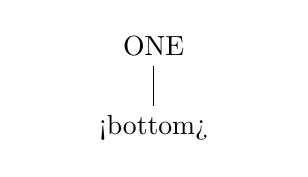
\begin{tikzpicture}
  [anchor=base]
  \node (bottom) at (0,0) {\isa{\\<bottom>}};
  \node (ONE) at (0,1) {\isa{ONE}};
  \draw (bottom) -- (ONE);
  \useasboundingbox (-1.6,0) -- (1.6,0);
  \end{tikzpicture}
}
\subfloat[\isa{tr = bool lift}]{
  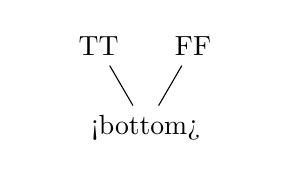
\begin{tikzpicture}
  [anchor=base]
  \node (bottom) at (0,0) {\isa{\\<bottom>}};
  \node (TT) at (-0.6,1) {\isa{TT}};
  \node (FF) at (0.6,1) {\isa{FF}};
  \draw (bottom) -- (TT);
  \draw (bottom) -- (FF);
  \useasboundingbox (-1.5,0) -- (1.5,0);
  \end{tikzpicture}
}
\subfloat[\isa{nat lift}]{
  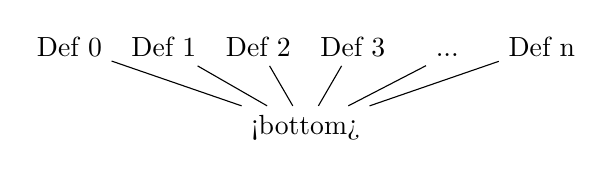
\begin{tikzpicture}
  [anchor=base]
  \node (bottom) at (0,0) {\isa{\\<bottom>}};
  \node (0) at (-3.0,1) {\isa{Def 0}};
  \node (1) at (-1.8,1) {\isa{Def 1}};
  \node (2) at (-0.6,1) {\isa{Def 2}};
  \node (3) at (0.6,1) {\isa{Def 3}};
  \node (dots) at (1.8,1) {\isa{...}};
  \node (n) at (3.0,1) {\isa{Def n}};
  \draw (bottom) -- (0);
  \draw (bottom) -- (1);
  \draw (bottom) -- (2);
  \draw (bottom) -- (3);
  \draw (bottom) -- (dots);
  \draw (bottom) -- (n);
  \end{tikzpicture}
}
\caption{Flat lifted types in HOLCF}
\label{fig:holcf-flat-types}
\end{figure}

\paragraph{Discrete cpo.} Any ordinary HOL type can be turned into a cpo by giving it a discrete ordering. In HOLCF this construction is formalized using the type \isa{'a discr}.

\indexdef{Discr}
\begin{isacode}
datatype 'a discr = Discr "'a"
\end{isacode}

\noindent
To go along with the constructor function \isa{Discr}, we define its inverse, \isa{undiscr}.

\indexdef{undiscr}
\begin{isacode}
definition undiscr :: "'a discr => 'a"
  where "undiscr x = (case x of Discr y => y)"
\end{isacode}
 
The ordering on type \isa{'a discr} is defined so that \isa{(x << y) = (x = y)}, which makes \isa{'a discr} an instance of the \isa{discrete_cpo} class (and thus also the \isa{chfin} class). In particular, this means that every function \isa{f :: 'a discr => 'b} is continuous, and every predicate \isa{P :: 'a discr => bool} is admissible.

It might make sense to define discrete orderings for various HOL types, such as \isa{bool}, \isa{nat}, and \isa{int}, making all those types instances of the \isa{discrete_cpo} class. However, this is not really necessary, because the types \isa{bool discr}, \isa{nat discr}, and \isa{int discr} can be used instead.

\HOLCF{11} does define a discrete ordering for the single-element HOL \isa{unit} type. Type \isa{unit} is special, because it is the only discrete cpo that also has a bottom element. For technical reasons, it is much simpler to make \isa{unit} an instance of class \isa{pcpo} directly than it would be to make \isa{unit discr :: pcpo}. The Isabelle type \isa{unit} corresponds to the \isa{void} type from Cambridge LCF \cite{paulson87lcf}.

\paragraph{Flat lifted type.} Any ordinary HOL type can be made into a pointed cpo by adjoining a new bottom element, and giving the new type a flat ordering (in the sense of the \isa{flat} type class described in Sec.~\ref{sec:holcf-classes}). This construction is formalized in HOLCF by the type \isa{'a lift}.

\begin{isacode}
pcpodef (open) 'a lift = "UNIV :: ('a discr)\<lifted> set"
\end{isacode}

\noindent
We use the \textsc{Cpodef} package to define \isa{'a lift} as an isomorphic copy of \isa{('a discr)\<lifted>}.\footnote{The \isa{(open)} option suppresses the definition of the set constant \isa{lift == UNIV}.}$^,$\footnote{Another sensible design choice would be to use \isa{type_synonym 'a lift = "'a discr u"}.} As such, the \isa{Rep_lift} and \isa{Abs_lift} functions form a continuous isomorphism. Next we define the constructor function, \isa{Def}.

\indexdef{Def}
\begin{isacode}
definition Def :: "'a => 'a lift"
  where "Def x = Abs_lift (up`(Discr x))"
\end{isacode}
%
Using this definition, we prove that \isa{Def} is injective and never returns \isa{\<bottom>}. It is also simple to prove an induction rule for type \isa{'a lift}, by case analysis on the representing type.

\indexthm{lift_induct}
\begin{isacode}
lemma lift_induct: "[|P \<bottom>; !!x. P (Def x)|] ==> P y"
\end{isacode}

\noindent
Using these lemmas, we then use the \isa{rep_datatype} command provided by the \textsc{Datatype} package to generate a case combinator \isa{lift_case} and various related theorems; thus we are allowed to treat \isa{Def} and \isa{\<bottom>} as constructors of an ordinary datatype.

By case analysis, and using the ordering properties of \isa{Def}, we can show that \isa{'a lift} is an instance of class \isa{flat}. Because \isa{flat} is a subclass of \isa{chfin}, this means also that every value of type \isa{'a lift} is compact.

In order to use \isa{lift_case} to define continuous functions, we need to prove a continuity rule for it. We start with a lemma that lets us express \isa{lift_case} using \isa{Rep_lift} and \isa{fup}. Having expressed \isa{lift_case} in terms of other continuous functions, it is now easy to show the continuity of \isa{lift_case}.

\indexthm{lift_case_eq}
\begin{isacode}
lemma lift_case_eq:
  "(case x of \<bottom> => \<bottom> | Def a => f a) = (case Rep_lift x of up`y => f (undiscr y))"
\end{isacode}
\unmedskip
\indexthm{cont2cont_lift_case}
\begin{isacode}
lemma cont2cont_lift_case [simp]:
  "[|!!a. cont (\<lambda>x. f x a); cont (\<lambda>x. g x)|]
    ==> cont (\<lambda>x. case g x of \<bottom> => \<bottom> | Def a => f x a)"
\end{isacode}

\noindent
To facilitate the definition of continuous functions on type \isa{'a lift}, we define combinators \isa{flift1} and \isa{flift2}. From \isa{cont2cont_lift_case}, we derive a continuity rule for \isa{flift1} (not shown).
\indexdef{flift1}
\begin{isacode}
definition flift1 :: "('a => 'b::pcpo) => ('a lift -> 'b)"
  where "flift1 f = (\<Lambda> x. case x of \<bottom> => \<bottom> | Def a => f a)"
\end{isacode}
\unmedskip
\indexdef{flift2}
\begin{isacode}
definition flift2 :: "('a => 'b) => ('a lift -> 'b lift)"
  where "flift2 f = flift1 (\<lambda>x. Def (f x))"
\end{isacode}
We also define the syntax \isa{(\<Lambda>(Def x). t)} to represent \isa{flift1 (\<lambda>x. t)}.

\paragraph{Lifted unit type.} We define the standard LCF type \isa{one} as a type synonym for \isa{unit lift}. We proceed to define the constructor \isa{ONE} and a case combinator \isa{one_case} (strict in its second argument), as shown. We also prove the expected ordering properties and rewrite rules for these constants.

\indexdef{type_synonym one}
\begin{isacode}
type_synonym one = "unit lift"
\end{isacode}
\unmedskip
\indexdef{ONE}
\begin{isacode}
definition ONE :: "one"
  where "ONE = Def ()"
\end{isacode}
\unmedskip
\indexdef{one_case}
\begin{isacode}
definition one_case :: "'a -> one -> 'a"
  where "one_case = (\<Lambda> x (Def u). x)"
\end{isacode}

\noindent
We define the syntax \isa{(case x of ONE => t)} to represent \isa{one_case`t`x}, and \isa{(\<Lambda> ONE. t)} to represent \isa{one_case`t}.

\paragraph{Lifted boolean type.} The LCF type of truth values, \isa{tr}, is defined as a synonym for \isa{bool lift}. This type has constructors \isa{TT} and \isa{FF}; its case combinator \isa{tr_case} is the continuous if-then-else operator.

\indexdef{type_synonym tr}
\begin{isacode}
type_synonym tr = "bool lift"
\end{isacode}
\unmedskip
\indexdef{TT}
\begin{isacode}
definition TT :: "tr"
  where "TT = Def True"
\end{isacode}
\unmedskip
\indexdef{FF}
\begin{isacode}
definition FF :: "tr"
  where "FF = Def False"
\end{isacode}
\unmedskip
\indexdef{tr_case}
\begin{isacode}
definition tr_case :: "'a -> 'a -> tr -> 'a"
  where "tr_case = (\<Lambda> x y (Def b). if b then x else y)"
\end{isacode}

\noindent
We define the syntax \isa{(If t then x else y)} to represent \isa{tr_case`x`y`t}. Note that we use ``\isa{If}'' with a capital letter to distinguish from the standard if-then-else operation on type \isa{bool}, which uses lowercase ``\isa{if}''.

%%%%%%%%%%%%%%%%%%%%%%%%%%%%%%%%%%%%%%%%%%%%%%%%%%%%%%%%%%%%%%%%%%%%%%

\subsection{Strict product type}
\label{sec:holcf-sprod}

The strict product (also known as ``smash product'') is one of the standard constructions in domain theory \cite{gunter90semantic, gunter92semantics, amadio+curien}. If $D$ and $E$ are pointed cpos, then $D \otimes E$ is also a pointed cpo. Its elements are strict pairs of the form $\llparenthesis x, y \rrparenthesis$, where $x \in D$ and $y \in E$. Strict pairs where either component equals $\bot$ are identified with the bottom element of $D \otimes E$, so that $\llparenthesis x, \bot \rrparenthesis = \llparenthesis \bot, y \rrparenthesis = \bot$.

In \HOLCF{11}, we define the strict product of \isa{'a} and \isa{'b} as a subset of the cartesian product type \isa{'a \<times> 'b}. The type consists of those pairs where neither element is \isa{\<bottom>}, plus the pair \isa{\<bottom> = (\<bottom>, \<bottom>)}.

\begin{isacode}
pcpodef ('a, 'b) sprod  (infixr "**" 20) =
  "{p::('a::pcpo \<times> 'b::pcpo). p = UU \<or> (fst p \<noteq> UU \<and> snd p \<noteq> UU)}"
\end{isacode}

\noindent
The proof obligations for \isa{pcpodef} are that the set contains \isa{UU}, and set membership is admissible. Both goals are solved immediately by simplification. (Note that as \isa{\<bottom>} is compact, being non-\isa{UU} is an admissible predicate.) The \textsc{Cpodef} package generates a set of lemmas analogous to those listed in Fig.~\ref{fig:holcf-cfun-cpodef}, plus a few more about the strictness of \isa{Rep_sprod} and \isa{Abs_sprod} (see Fig.~\ref{fig:holcf-sprod-pcpodef}).

\begin{figure}
\indexdef{sprod}
\indexthm{Rep_sprod_inverse}
\indexthm{Abs_sprod_inverse}
\indexthm{Rep_sprod}
\indexthm{Rep_sprod_inject}
\indexthm{below_sprod_def}
\indexthm{cont_Rep_sprod}
\indexthm{cont_Abs_sprod}
\indexthm{compact_sprod}
\indexthm{Rep_sprod_strict}
\indexthm{Abs_sprod_strict}
\begin{isabelle}
definition sprod_def: "sprod \<equiv> {p. p = UU \<or> (fst p ~= UU \<and> snd p ~= UU)}"
theorem Rep_sprod_inverse: "Abs_sprod (Rep_sprod x) = x"
theorem Abs_sprod_inverse: "y \<in> sprod ==> Rep_sprod (Abs_sprod y) = y"
theorem Rep_sprod: "Rep_sprod x \<in> sprod"
theorem Rep_sprod_inject: "(Rep_sprod x = Rep_sprod y) = (x = y)"
definition below_sprod_def: "(op \<sqsubseteq>) \<equiv> (\<lambda>x y. Rep_sprod x \<sqsubseteq> Rep_sprod y)"
theorem cont_Rep_sprod: "cont f ==> cont (\<lambda>x. Rep_sprod (f x))"
theorem cont_Abs_sprod: "[|!!x. f x \<in> sprod; cont f|] ==> cont (\<lambda>x. Abs_sprod (f x))"
theorem compact_sprod: "compact (Rep_sprod x) ==> compact x"
theorem Rep_sprod_strict: "Rep_sprod \<bottom> = \<bottom>"
theorem Abs_sprod_strict: "Abs_sprod \<bottom> = \<bottom>"
\end{isabelle}
\caption{Selected theorems generated by \isa{pcpodef} for strict product type}
\label{fig:holcf-sprod-pcpodef}
\end{figure}

\paragraph{Constructor function.} The first operation we define is the strict pair constructor, \isa{spair}. The definition uses the operator \isa{seq} to ensure that if either \isa{a} or \isa{b} is \isa{\<bottom>}, then both components of the resulting pair will be \isa{\<bottom>}.

\indexdef{spair}
\begin{isacode}
definition spair :: "'a -> 'b -> ('a ** 'b)"
  where "spair = (\<Lambda> a b. Abs_sprod (seq`b`a, seq`a`b))"
\end{isacode}

\noindent
We also define syntax for strict tuples. The expression \isa{(:a, b:)} is syntax for \isa{spair`a`b}; larger tuples nest to the right, so \isa{(:a, b, c:)} means \isa{spair`a`(spair`b`c)}.
 
In order to prove properties about \isa{spair}, we need to know how \isa{Rep_sprod} acts on it. We start by proving \isa{(seq`b`a, seq`a`b) \<in> sprod} as a lemma. Then we can use \isa{cont_Abs_sprod} and \isa{Abs_sprod_inverse} (provided by the \textsc{Cpodef} package) to beta-reduce the definition of \isa{spair} and prove the desired rule:

\indexthm{Rep_sprod_spair}
\begin{isacode}
lemma Rep_sprod_spair: "Rep_sprod (:a, b:) = (seq`b`a, seq`a`b)"
\end{isacode}

\noindent
Together with a group of other rewrite rules, the lemma \isa{Rep_sprod_spair} forms part of a general strategy for proving properties about strict products. The rules in \isa{Rep_sprod_simps} replace comparisons on type \isa{'a ** 'b} with comparisons on the component types \isa{'a} and \isa{'b}.

\indexthm{Rep_sprod_simps}
\begin{isacode}
lemma Rep_sprod_simps:
  "x = y <-> Rep_sprod x = Rep_sprod y"
  "x << y <-> Rep_sprod x << Rep_sprod y"
  "t = u <-> fst t = fst u & snd t = snd u"
  "t << u <-> fst t << fst u & snd t << snd u"
  "Rep_sprod (:a, b:) = (seq`b`a, seq`a`b)"
  "Rep_sprod UU = UU"
\end{isacode}

\noindent
Each of the following five lemmas is proved automatically by simplifying with \isa{Rep_sprod_simps}. (The if-and-only-if rules also require \isa{seq_conv_if}, so that the simplifier will do the appropriate case splits on whether or not values equal \isa{UU}.)

\indexthm{spair_strict1}
\begin{isacode}
lemma spair_strict1 [simp]: "(:\<bottom>, b:) = \<bottom>"
\end{isacode}
\unmedskip
\indexthm{spair_strict2}
\begin{isacode}
lemma spair_strict2 [simp]: "(:a, \<bottom>:) = \<bottom>"
\end{isacode}
\unmedskip
\indexthm{spair_bottom_iff}
\begin{isacode}
lemma spair_bottom_iff [simp]: "(:a, b:) = \<bottom> <-> a = \<bottom> \<or> b = \<bottom>"
\end{isacode}
\unmedskip
\indexthm{spair_below_iff}
\begin{isacode}
lemma spair_below_iff: "(:a, b:) << (:c, d:) <->
  a = \<bottom> \<or> b = \<bottom> \<or> (a << c \<and> b << d)"
\end{isacode}
\unmedskip
\indexthm{spair_eq_iff}
\begin{isacode}
lemma spair_eq_iff: "(:a, b:) = (:c, d:) <->
  (a = c \<and> b = d) \<or> ((a = \<bottom> \<or> b = \<bottom>) \<and> (c = \<bottom> \<or> d = \<bottom>))"
\end{isacode}

The same set of rewrite rules also works for proving a case analysis rule for type \isa{'a ** 'b}. The proof of \isa{sprodE} starts by inserting the fact \isa{Rep_sprod y \<in> sprod} into the goal state. Then we unfold the definition of \isa{sprod}, and use the \isa{auto} tactic to split the disjunctions and simplify.
%
\indexthm{sprodE}
\begin{isacode}
lemma sprodE:
  "[|y = UU ==> P; !!a b. [|y = (:a, b:); a ~= UU; b ~= UU|] ==> P|] ==> P"
\end{isacode}
%
The induction rule for strict products is a direct consequence of the case analysis rule.
%
\indexthm{sprod_induct}
\begin{isacode}
lemma sprod_induct: "[|P UU; !!a b. [|a ~= UU; b ~= UU|] ==> P (:a, b:)|] ==> P x"
\end{isacode}

One more useful rule about \isa{spair} concerns compactness. We can use the lemma \isa{compact_sprod} provided by the \textsc{Cpodef} package together with \isa{Rep_sprod_spair} to prove the following rule.
%
\indexthm{compact_spair}
\begin{isacode}
lemma compact_spair: "[|compact a; compact b|] ==> compact (:a, b:)"
\end{isacode}
\unmedskip

\paragraph{Projections.} After the constructor \isa{spair}, the next functions we define are the projections \isa{sfst} and \isa{ssnd}. We can easily unfold and beta-reduce their definitions, because \isa{fst}, \isa{snd}, and \isa{Rep_sprod} are all known to be continuous.
\indexdef{sfst}
\begin{isacode}
definition sfst :: "('a ** 'b) -> 'a"
  where "sfst = (\<Lambda> p. fst (Rep_sprod p))"
\end{isacode}
\unmedskip
\indexdef{ssnd}
\begin{isacode}
definition ssnd :: "('a ** 'b) -> 'b"
  where "ssnd = (\<Lambda> p. snd (Rep_sprod p))"
\end{isacode}
The basic properties of \isa{sfst} and \isa{ssnd} can be proven by beta-reducing their definitions, and simplifying with \isa{Rep_sprod_simps}.
\indexthm{sfst_strict}
\indexthm{ssnd_strict}
\indexthm{sfst_spair}
\indexthm{ssnd_spair}
\begin{isacodes}
lemma sfst_strict [simp]: "sfst`UU = UU"
lemma ssnd_strict [simp]: "ssnd`UU = UU"
lemma sfst_spair [simp]: "y ~= UU ==> sfst`(:x, y:) = x"
lemma ssnd_spair [simp]: "x ~= UU ==> ssnd`(:x, y:) = y"
\end{isacodes}
\unmedskip

\paragraph{Case combinator.} The last operation on strict products that we need to define is the case combinator, \isa{ssplit}.
\indexdef{ssplit}
\begin{isacode}
definition ssplit :: "('a -> 'b -> 'c) -> ('a ** 'b) -> 'c"
  where "ssplit = (\<Lambda> f p. seq`p`(f`(sfst`p)`(ssnd`p)))"
\end{isacode}
The characteristic lemmas for \isa{ssplit} are proved easily by unfolding the definition. Note that the use of \isa{seq} in the definition of \isa{ssplit} is needed for the strictness rule to hold.
\indexthm{ssplit_simps}
\begin{isacode}
lemma ssplit_simps [simp]:
  "ssplit`f`UU = UU"
  "[|x ~= UU; y ~= UU|] ==> ssplit`f`(:x, y:) = f`x`y"
\end{isacode}
The syntax \isa{(case x of (:a, b:) => t)} stands for \isa{ssplit`(\<Lambda> a b. t)`x}. We also support lambda syntax: \isa{(\<Lambda> (:a, b:). t)} is shorthand for \isa{ssplit`(\<Lambda> a b. t)}. Larger tuples work too; for example, \isa{(\<Lambda> (:a, b, c:). t)} translates to \isa{ssplit`(\<Lambda> a. ssplit`(\<Lambda> b c. t))}.

%%%%%%%%%%%%%%%%%%%%%%%%%%%%%%%%%%%%%%%%%%%%%%%%%%%%%%%%%%%%%%%%%%%%%%

\subsection{Strict sum type}
\label{sec:holcf-ssum}

The strict sum $D \oplus E$ (also known as ``smash sum'' or ``coalesced sum'') is another standard construction in domain theory \cite{gunter90semantic, gunter92semantics, amadio+curien}. If $D$ and $E$ are pointed cpos, then $D \oplus E$ is also a pointed cpo. There are continuous injections $\iota_1 : D \to D \oplus E$ and $\iota_2 : E \to D \oplus E$, similar to the disjoint sum. But unlike the disjoint sum, we identify the bottom elements injected from $D$ and $E$, making each injection strict: $\iota_1(\bot) = \iota_2(\bot) = \bot$ (see Fig.~\ref{fig:holcf-strict-sum}).

\begin{figure}
\centering
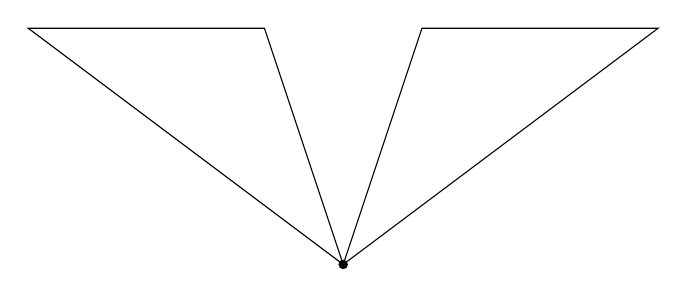
\begin{tikzpicture}
  [anchor=base]
  \draw (0,0) -- (4,3) -- (1,3) -- cycle;
  \draw (0,0) -- (-4,3) -- (-1,3) -- cycle;
  \fill (0,0) circle (0.06);
\end{tikzpicture}
\caption{Strict sum of pointed cpos}
\label{fig:holcf-strict-sum}
\end{figure}

In \HOLCF{11}, we define the strict sum of \isa{'a} and \isa{'b} as a set of triples of type \isa{(tr \<times> 'a \<times> 'b)}. The first component is a tag specifying whether the value should be interpreted as a left- or right-injection. Depending on the value of the tag, the injected value is stored in either the second or third slot, with the other slot containing \isa{\<bottom>}. The bottom element of the strict sum type is represented as \isa{\<bottom> = (\<bottom>, \<bottom>, \<bottom>)}.

\begin{isacode}
pcpodef ('a, 'b) ssum (infixr "++" 10) = 
  "{p :: (tr \<times> 'a::pcpo \<times> 'b::pcpo). p = \<bottom> \<or>
      (fst p = TT \<and> fst (snd p) \<noteq> \<bottom> \<and> snd (snd p) = \<bottom>) \<or>
      (fst p = FF \<and> fst (snd p) = \<bottom> \<and> snd (snd p) \<noteq> \<bottom>) }"
\end{isacode}

\noindent
The proof obligations for \isa{pcpodef} are that the set contains \isa{UU}, and set membership is admissible. As with the strict product, both goals are solved immediately by simplification. For the strict sum type, the \textsc{Cpodef} package provides a set of theorems just like the ones shown in Fig.~\ref{fig:holcf-sprod-pcpodef} for strict product; we omit the strict sum versions here.

\paragraph{Constructor functions.} After defining the type, we can define the constructor functions \isa{sinl} and \isa{sinr}.\footnote{The names of \isa{sinl} and \isa{sinr} come from earlier versions of LCF; respectively they stand for ``\emph{s}trict-\emph{in}jection-\emph{l}eft'' and ``\emph{s}trict-\emph{in}jection-\emph{r}ight''.} Because both constructor functions are supposed to be strict, we use the \isa{seq} operator to ensure that the tag component is \isa{UU} whenever the constructor argument is \isa{UU}.

\indexdef{sinl}
\begin{isacode}
definition sinl :: "'a -> ('a ++ 'b)"
  where "sinl = (\<Lambda> a. Abs_ssum (seq`a`TT, a, \<bottom>))"
\end{isacode}
\unmedskip
\indexdef{sinr}
\begin{isacode}
definition sinr :: "'b -> ('a ++ 'b)"
  where "sinr = (\<Lambda> b. Abs_ssum (seq`b`FF, \<bottom>, b))"
\end{isacode}

Similarly to the strict product, the next thing we must do is prove how \isa{Rep_ssum} acts on the constructors. After proving lemmas to the effect that \isa{(seq`a`TT, a, \<bottom>)} and \isa{(seq`b`FF, \<bottom>, b)} are always in the set \isa{ssum}, we can use \isa{cont_Abs_ssum} and \isa{Abs_ssum_inverse} to derive the following two rules.

\indexthm{Rep_ssum_sinl}
\indexthm{Rep_ssum_sinr}
\begin{isacodes}
lemma Rep_ssum_sinl: "Rep_ssum (sinl`a) = (seq`a`TT, a, \<bottom>)"
lemma Rep_ssum_sinr: "Rep_ssum (sinr`b) = (seq`b`FF, \<bottom>, b)"
\end{isacodes}

\noindent
These are combined with other lemmas about \isa{Rep_ssum} to form \indexthm{Rep_ssum_simps}\isa{Rep_ssum_simps}, which is the strict-sum analog of \isa{Rep_sprod_simps} from the previous section. This set of rewrite rules lets us reduce comparisons on type \isa{'a ++ 'b} to comparisons on types \isa{tr}, \isa{'a} and \isa{'b}. We can use them (together with \isa{seq_conv_if}, as needed) to prove the complete set of simplification rules for \isa{sinl} and \isa{sinr} shown in Fig.~\ref{fig:holcf-sinl-sinr}.

\begin{figure}
\indexthm{sinl_below}
\indexthm{sinr_below}
\indexthm{sinl_below_sinr}
\indexthm{sinr_below_sinl}
\begin{minipage}{0.275\linewidth}
\begin{isabelle}
lemma sinl_below
lemma sinr_below
lemma sinl_below_sinr
lemma sinr_below_sinl
\end{isabelle}
\end{minipage}
\begin{minipage}{0.7\linewidth}
\begin{isabelle}
[simp]: "(sinl`x \<sqsubseteq> sinl`y) = (x \<sqsubseteq> y)"
[simp]: "(sinr`x \<sqsubseteq> sinr`y) = (x \<sqsubseteq> y)"
[simp]: "(sinl`x \<sqsubseteq> sinr`y) = (x = \<bottom>)"
[simp]: "(sinr`x \<sqsubseteq> sinl`y) = (x = \<bottom>)"
\end{isabelle}
\end{minipage}

\indexthm{sinl_eq}
\indexthm{sinr_eq}
\indexthm{sinl_eq_sinr}
\indexthm{sinr_eq_sinl}
\begin{minipage}{0.275\linewidth}
\begin{isabelle}
lemma sinl_eq
lemma sinr_eq
lemma sinl_eq_sinr
lemma sinr_eq_sinl
\end{isabelle}
\end{minipage}
\begin{minipage}{0.7\linewidth}
\begin{isabelle}
[simp]: "(sinl`x = sinl`y) = (x = y)"
[simp]: "(sinr`x = sinr`y) = (x = y)"
[simp]: "(sinl`x = sinr`y) = (x = \<bottom> \<and> y = \<bottom>)"
[simp]: "(sinr`x = sinl`y) = (x = \<bottom> \<and> y = \<bottom>)"
\end{isabelle}
\end{minipage}

\indexthm{sinl_strict}
\indexthm{sinr_strict}
\indexthm{sinl_bottom_iff}
\indexthm{sinr_bottom_iff}
\begin{minipage}{0.275\linewidth}
\begin{isabelle}
lemma sinl_strict
lemma sinr_strict
lemma sinl_bottom_iff
lemma sinr_bottom_iff
\end{isabelle}
\end{minipage}
\begin{minipage}{0.7\linewidth}
\begin{isabelle}
[simp]: "sinl`\<bottom> = \<bottom>"
[simp]: "sinr`\<bottom> = \<bottom>"
[simp]: "(sinl`x = \<bottom>) = (x = \<bottom>)"
[simp]: "(sinr`x = \<bottom>) = (x = \<bottom>)"
\end{isabelle}
\end{minipage}
\caption{Order, injectivity, distinctness, and strictness of \isa{sinl} and \isa{sinr}}
\label{fig:holcf-sinl-sinr}
\end{figure}
 
The same rewrites are also sufficient to prove the case analysis rule for the strict sum type. Starting with the fact \isa{Rep_ssum y \<in> ssum} (a theorem provided by \textsc{Cpodef}), we can unfold the definition of \isa{ssum} and then use \isa{Rep_ssum_simps} with the \isa{auto} tactic to complete the proof.

\indexthm{ssumE}
\begin{isacode}
lemma ssumE: "[|y = UU ==> P;
  !!a. [|y = sinl`a; a ~= UU|] ==> P; !!b. [|y = sinr`b; b ~= UU|] ==> P|] ==> P"
\end{isacode}

\noindent
The induction rule for strict sums is a direct consequence of the case analysis rule.

\indexthm{ssum_induct}
\begin{isacode}
lemma ssum_induct:
  "[|P UU; !!a. a ~= UU ==> P (sinl`a); !!b. b ~= UU ==> P (sinr`b)|] ==> P x"
\end{isacode}

We can prove if-and-only-if compactness rules for \isa{sinl} and \isa{sinr}. For the ($\Longleftarrow$) direction, we use a compactness rule provided by \textsc{Cpodef}: A value of type \isa{'a \<oplus> 'b} is compact if its representation in type \isa{tr \<times> 'a \<times> 'b} is compact. The proof of the ($\Longrightarrow$) direction uses the definition of compactness and the \isa{adm_subst} rule. We assume \isa{compact (sinl`a)}, which means \isa{adm (\<lambda>x. sinl`a \<notsqsubseteq> x)}; this implies \isa{adm (\<lambda>x. sinl`a \<notsqsubseteq> sinl`x)}, which simplifies to \isa{adm (\<lambda>x. a \<notsqsubseteq> x)}, which is the definition of \isa{compact a}. The proof for \isa{sinr} is identical.

\indexthm{compact_sinl_iff}
\indexthm{compact_sinr_iff}
\begin{isacodes}
lemma compact_sinl_iff [simp]: "compact (sinl`a) = compact a"
lemma compact_sinr_iff [simp]: "compact (sinr`b) = compact b"
\end{isacodes}
\unmedskip

\paragraph{Case combinator.} Besides the constructors \isa{sinl} and \isa{sinr}, the other basic operation on strict sums is the case combinator, \isa{sscase}. The definition uses \isa{Rep_ssum} to examine its argument, and the continuous if-then-else operation on type \isa{tr} to select which branch to take.
\indexdef{sscase}
\begin{isacode}
definition sscase :: "('a -> 'c) -> ('b -> 'c) -> ('a ++ 'b) -> 'c"
  where "sscase = (\<Lambda> f g s. (\<lambda>(t, x, y). If t then f`x else g`y) (Rep_ssum s))"
\end{isacode}
Using lemma \isa{cont_Rep_ssum} from the \textsc{Cpodef} package, it is easy to show that the abstractions used in the definition of \isa{sscase} are continuous. Proving the characteristic properties of \isa{sscase} is a simple matter of beta-reducing the definition and simplifying with \isa{Rep_ssum_simps}.
\indexthm{sscase_simps}
\begin{isacode}
lemma sscase_simps [simp]:
  "sscase`f`g`\<bottom> = \<bottom>"
  "x \<noteq> \<bottom> ==> sscase`f`g`(sinl`x) = f`x"
  "y \<noteq> \<bottom> ==> sscase`f`g`(sinr`y) = g`y"
\end{isacode}
As with the other case combinators, we define special syntax for \isa{sscase}. The term \isa{sscase`(\<Lambda> a. t)`(\<Lambda> b. u)`x} is rendered as \isa{(case x of sinl`a => t | sinr`b => u)}.


%%%%%%%%%%%%%%%%%%%%%%%%%%%%%%%%%%%%%%%%%%%%%%%%%%%%%%%%%%%%%%%%%%%%%%

\section{Automating continuity proofs}
\label{sec:holcf-automation}

When reasoning in HOLCF, continuity goals pop up all the time: Every beta-reduction of a continuous function abstraction requires a continuity proof. Continuity proofs are also needed, for example, to show admissibility of predicates like \isa{(\<lambda>x. f x << g x)}. Because they occur so often in practice, it is important that continuity proofs be both automatic and efficient---they should involve a minimal number of proof steps, and be processed in a short amount of time.

In this section we discuss three alternative proof techniques for continuity, starting with the method used by previous versions of HOLCF. Following this, we introduce two novel proof methods for continuity, each of which offers improved efficiency in terms of number of proof steps and running time.

\subsection{Original HOLCF continuity tactic}

\HOLCF{95} introduced a continuity tactic that repeatedly applied the following four continuity lemmas:

\indexthm{cont_id}
\begin{isacode}
lemma cont_id: "cont (\<lambda>x. x)"
\end{isacode}
\unmedskip
\indexthm{cont_const}
\begin{isacode}
lemma cont_const: "cont (\<lambda>x. c)"
\end{isacode}
\unmedskip
\indexthm{cont2cont_APP}
\begin{isacode}
lemma cont2cont_APP:
  "[|cont (\<lambda>x. f x); cont (\<lambda>x. t x)|] ==> cont (\<lambda>x. (f x)`(t x))"
\end{isacode}
\unmedskip
\indexthm{cont2cont_LAM}
\begin{isacode}
lemma cont2cont_LAM:
  "[|\<And>x. cont (\<lambda>y. f x y); \<And>y. cont (\<lambda>x. f x y)|] ==> cont (\<lambda>x. \<Lambda> y. f x y)"
\end{isacode}

If we add these four rules to the simplifier, then we will be able to prove continuity automatically for any term written in the LCF sub-language---i.e., any term consisting of continuous applications, continuous abstractions, and variables and constants with continuous function types. Looking at the forms of the rules, we can see that the terms in the assumptions are all strictly smaller than the terms in the conclusions, showing that the process of applying rules must eventually terminate.

But while the proofs may be automatic, they are not efficient. The problem lies specifically with the rule \isa{cont2cont_LAM}. Consider what happens when we have a term with multiple nested function abstractions (see Fig.~\ref{fig:holcf-cont-slow}). After repeatedly applying rule \isa{cont2cont_LAM} as many times as possible, we are left with \emph{eight} subgoals. In fact, the number of subgoals is equal to $2^n$, where $n$ is the number of nested lambdas.

\begin{figure}
\begin{singlespace}
\begin{isabelle}
lemma "cont (%x. \<Lambda> a b c. f`a`b`c`x)"
  apply (intro cont2cont_LAM)

 goal (8 subgoals):
 1. !!x a b. cont (%c. f`a`b`c`x)
 2. !!x a c. cont (%b. f`a`b`c`x)
 3. !!x b a. cont (%c. f`a`b`c`x)
 4. !!x b c. cont (%a. f`a`b`c`x)
 5. !!a x b. cont (%c. f`a`b`c`x)
 6. !!a x c. cont (%b. f`a`b`c`x)
 7. !!a b x. cont (%c. f`a`b`c`x)
 8. !!a b c. cont (%x. f`a`b`c`x)
\end{isabelle}
\end{singlespace}
\caption{Exponential blow-up using rule \isa{cont2cont_LAM}}
\label{fig:holcf-cont-slow}
\end{figure}

However, it is immediately evident that many of these subgoals are really the same; there are only $(n+1)$ distinct subgoals, each requiring continuity with respect to a different variable. This suggests the possibility of solving continuity goals in less than an exponential number of steps.

\subsection{Bottom-up continuity proofs}

One possible strategy is to work bottom-up: First prove continuity for the small subterms, and then combine those proofs to get continuity over the larger terms. Note that this is basically opposite to the introduction-rules approach, which works top-down. For each subterm, we construct a list of continuity theorems, one for each bound variable that occurs free in the subterm. For example, when proving \isa{cont (\<lambda>x. \<Lambda> a b c. f`a`b`c`x)}, the subterm \isa{(\<Lambda> c. f`a`b`c`x)} will have continuity theorems for the variables \isa{a}, \isa{b} and \isa{x} (shown in Fig.~\ref{fig:holcf-cont-algorithm} as \isa{a5}, \isa{b5}, and \isa{x5}). We treat \isa{f} like a constant, because it is free in the original goal.

\begin{figure}
\begin{singlespace}
\begin{isabelle}
have a0: "cont (%a. a)" by (rule cont_id)
from cont_const a0 have a1: "cont (%a. f`a)" by (rule cont2cont_APP)
from a1 cont_const have a2: "!!b. cont (%a. f`a`b)" by (rule cont2cont_APP)

...

from ... have a4: "!!b c x. cont (%a. f`a`b`c`x)" by (rule cont2cont_APP)
from ... have b4: "!!a c x. cont (%b. f`a`b`c`x)" by (rule cont2cont_APP)
from ... have c4: "!!a b x. cont (%c. f`a`b`c`x)" by (rule cont2cont_APP)
from ... have x4: "!!a b c. cont (%x. f`a`b`c`x)" by (rule cont2cont_APP)

from c4 and a4 have a5: "!!b x. cont (%a. \<Lambda> c. f`a`b`c`x)" by (rule cont2cont_LAM)
from c4 and b4 have b5: "!!a x. cont (%b. \<Lambda> c. f`a`b`c`x)" by (rule cont2cont_LAM)
from c4 and x4 have x5: "!!a b. cont (%x. \<Lambda> c. f`a`b`c`x)" by (rule cont2cont_LAM)
 
from b5 and a5 have a6: "!!x. cont (%a. \<Lambda> b c. f`a`b`c`x)" by (rule cont2cont_LAM)
from b5 and x5 have x6: "!!a. cont (%x. \<Lambda> b c. f`a`b`c`x)" by (rule cont2cont_LAM)

from a6 and x6 have x7: "cont (%x. \<Lambda> a b c. f`a`b`c`x)" by (rule cont2cont_LAM)
\end{isabelle}
\end{singlespace}
\caption{Bottom-up algorithm for proving continuity, using forward proof}
\label{fig:holcf-cont-algorithm}
\end{figure}

Next we move up to the next larger subterm, \isa{(\<Lambda> b c. f`a`b`c`x)}, which gets continuity theorems for the variables \isa{a} and \isa{x} (shown as \isa{a6} and \isa{x6}). Each of the new continuity theorems is derived from two earlier ones using the rule \isa{cont2cont_LAM}. Note that rule \isa{b5} is used more than once; such re-use prevents the exponential blow-up that we had before.

The bottom-up algorithm is now implemented in \HOLCF{11} (\texttt{HOLCF/Tools{\slash}cont\_proc.ML}). It has the advantage of being fast: It solves continuity subgoals using a small number of rule applications (quadratic in the number of nested lambdas, rather than exponential). Another advantage is that without any extra work, the algorithm can return a whole list of continuity theorems that it proved for subterms. This is useful for doing multiple beta-reductions, for example when proving something like \isa{(\<Lambda> a b c. f`a`b`c`x)`u`v`w = f`u`v`w`x}. This technique is used successfully by the \textsc{Domain} package for internal proofs, where large subgoals of this form arise from large datatype definitions (see Sec.~\ref{sec:domain-implementation}).

Compared to using introduction rules, the main disadvantage of the bottom-up algorithm is that it is difficult to extend the system to handle new constants. For example, when M\"{u}ller introduced the \isa{lift} type to allow mixing HOL and LCF terms, he was able to extend the continuity tactic by simply adding a couple of new rules, such as the one below for \isa{lift_case} \cite[\S5.2.2]{mueller98thesis} \cite[\S4.3.2]{hol+lcf}.
%
\indexthm{cont2cont_lift_case}
\begin{isacode}
lemma cont2cont_lift_case:
  "[|!!y. cont (\<lambda>x. f x y); cont (\<lambda>x. g x)|]
    ==> cont (\<lambda>x. case g x of \<bottom> => \<bottom> | Def y => f x y)"
\end{isacode}
%
Similarly, we have continuity rules for operations on the HOL product type:
%
\indexthm{cont2cont_Pair}
\begin{isacode}
lemma cont2cont_Pair:
  "[|cont (\<lambda>x. f x); cont (\<lambda>x. g x)|] ==> cont (\<lambda>x. (f x, g x))"
\end{isacode}
\unmedskip
\indexthm{cont2cont_prod_case}
\begin{isacode}
lemma cont2cont_prod_case:
  "[|!!a b. cont (\<lambda>x. f x a b); !!x b. cont (\<lambda>a. f x a b);
    !!x a. cont (\<lambda>b. f x a b); cont (\<lambda>x. g x)|]
    ==> cont (\<lambda>x. case g x of (a, b) => f x a b)"
\end{isacode}
%
An ideal continuity prover should allow users to add support for new constants by adding such rules. But as implemented, the bottom-up continuity algorithm is not so easily extensible. Properly supporting rules like \isa{cont2cont_prod_case} is especially troublesome because, like \isa{cont2cont_LAM}, it has multiple hypotheses for the same subterm, and would require similar handling to avoid an exponential blow-up. Yet the rule has a different form than \isa{cont2cont_LAM}. A single algorithm that could handle the full range of possibilities for such rules would have to be rather sophisticated.

\subsection{Efficient continuity rules using products}

As it turns out, it is possible to design an extensible set of continuity introduction rules that avoids the exponential blow-up inherent in the original \HOLCF{95} continuity tactic. The key to designing these rules is a property of continuous functions $f : D \times E \to F$. It is a standard result in domain theory that a function on a product type is continuous if and only if it is continuous in each component separately \cite[Lemma 3.2.6]{abramsky94domain}. This property is formalized in the \HOLCF{11} theory of products as lemma \isa{prod_cont_iff}.
%
\indexthm{prod_cont_iff}
\begin{isacode}
lemma prod_cont_iff:
  "cont f <-> (\<forall>y. cont (\<lambda>x. f (x, y))) \<and> (\<forall>x. cont (\<lambda>y. f (x, y)))"
\end{isacode}
%
We can use this theorem to combine the two premises of the \isa{cont2cont_LAM} rule into one. Compare the two versions of this rule:
%
\indexthm{cont2cont_LAM}
\begin{isacode}
lemma cont2cont_LAM:
  "[|\<And>x. cont (\<lambda>y. f x y); \<And>y. cont (\<lambda>x. f x y)|] ==> cont (\<lambda>x. \<Lambda> y. f x y)"
\end{isacode}
\unmedskip
\indexthm{cont2cont_LAM'}
\begin{isacode}
lemma cont2cont_LAM':
  "cont (\<lambda>p. f (fst p) (snd p)) ==> cont (\<lambda>x. \<Lambda> y. f x y)"
\end{isacode}
%
We can evaluate the behavior of the new \isa{cont2cont_LAM'} rule by considering the same continuity goal we used before in Fig.~\ref{fig:holcf-cont-slow}. After applying the continuity rule \isa{cont2cont_LAM'} three times, we are now left with just a single subgoal (see Fig.~\ref{fig:holcf-cont-fast}). The remaining goal can be solved by applying standard continuity rules (\isa{cont_id}, \isa{cont_const}, and \isa{cont2cont_APP}) together with continuity rules for \isa{fst} and \isa{snd}. The complete set of rules (which we call \isa{cont2cont} rules) for proving continuity of LCF terms is shown in Fig.~\ref{fig:holcf-cont2cont-rules}. All of them are safe to add to the Isabelle simplifier.

\begin{figure}
\begin{singlespace}
\begin{isabelle}
lemma "cont (%x. \<Lambda> a b c. f`a`b`c`x)"
  apply (intro cont2cont_LAM')
 
goal (1 subgoal):
 1. cont (%p. f`(snd (fst (fst p)))`(snd (fst p))`(snd p)`(fst (fst (fst p))))
\end{isabelle}
\end{singlespace}
\caption{Efficient behavior of continuity introduction rule \isa{cont2cont_LAM'}}
\label{fig:holcf-cont-fast}
\end{figure}

\begin{figure}
\begin{isacode}
lemma cont_id [simp]: "cont (\<lambda>x. x)"
\end{isacode}
\unmedskip
\begin{isacode}
lemma cont_const [simp]: "cont (\<lambda>x. c)"
\end{isacode}
\unmedskip
\begin{isacode}
lemma cont2cont_fst [simp]: "cont (%x. f x) ==> cont (%x. fst (f x))"
\end{isacode}
\unmedskip
\begin{isacode}
lemma cont2cont_snd [simp]: "cont (%x. f x) ==> cont (%x. snd (f x))"
\end{isacode}
\unmedskip
\begin{isacode}
lemma cont2cont_APP [simp]:
  "[|cont (\<lambda>x. f x); cont (\<lambda>x. t x)|] ==> cont (\<lambda>x. (f x)`(t x))"
\end{isacode}
\unmedskip
\begin{isacode}
lemma cont2cont_LAM' [simp]:
  "cont (\<lambda>p. f (fst p) (snd p)) ==> cont (\<lambda>x. \<Lambda> y. f x y)"
\end{isacode}
\caption{Complete set of efficient \isa{cont2cont} rules for LCF terms}
\label{fig:holcf-cont2cont-rules}
\end{figure}

Unlike rule \isa{cont2cont_LAM}, each rule in Fig.~\ref{fig:holcf-cont2cont-rules} has only one continuity premise for each subterm. Proving continuity with this set of rules requires more than a linear number of steps, though, because as lambdas are eliminated, the subgoal grows to a larger size: \isa{fst} and \isa{snd} are introduced on every bound variable. But the size increase is not exponential; it is merely quadratic in the number of nested lambdas. So, like the bottom-up algorithm, the \isa{cont2cont} rules can discharge a continuity goal with nested lambdas in a quadratic number of steps. In practice, the run-time efficiency of the \isa{cont2cont} rules is about the same as for the bottom-up continuity tactic. (Either can discharge a continuity goal with twenty nested lambdas in a fraction of a second, and the total run-time for each seems to be $O(n^3)$.)

The \isa{cont2cont} rules are easily extensible. We can add new rules to the simplifier for each new constant we want (such as \isa{cont2cont_lift_case}) without any trouble. For constants like \isa{prod_case}, whose continuity rules require continuity of multiple variables over the same subterm, we can use \isa{prod_cont_iff} to derive an efficient version of the rule, just like we did for \isa{cont2cont_LAM}. For example, here is the efficient \isa{cont2cont} rule for \isa{prod_case}:

\indexthm{cont2cont_prod_case'}
\begin{isacode}
lemma cont2cont_prod_case' [simp]:
  "[|cont (%p. f (fst p) (fst (snd p)) (snd (snd p))); cont (%x. g x)|]
    ==> cont (%x. case g x of (a, b) => f x a b)"
\end{isacode}

For organizing continuity introduction rules, \HOLCF{11} provides a special \isa{cont2cont} theorem attribute. Declaring a lemma with \isa{[cont2cont]} dynamically adds it to a list of theorems, which is also referred to by the name \isa{cont2cont}. (Typically each \isa{cont2cont} rule should also be added to the simplifier.) Users can then do continuity proofs with the proof method ``\isa{intro cont2cont}''.

Using ``\isa{intro cont2cont}'' is a bit faster (by about a factor of two) than calling ``\isa{simp}'' on a continuity goal, because it has a smaller, targeted set of rules, and avoids deep recursive calls to the simplifier. To take advantage of this speedup in the common case, \HOLCF{11} defines a special simplification procedure (or ``simproc'') for the beta reduction rule:

\indexthm{beta_cfun}
\begin{isacode}
lemma beta_cfun: "cont f ==> (\<Lambda> x. f x)`u = f u"
\end{isacode}

\noindent
In \HOLCF{11}, \isa{beta_cfun} is not declared with the \isa{[simp]} attribute. Instead, the simplifier is configured to call a certain simproc when it sees a term matching the pattern \isa{(\<Lambda> x. f x)`u}. When the simproc is run, it tries to prove the goal \isa{cont f} using the proof method ``\isa{intro cont2cont}''. If the subproof succeeds, the simproc returns the unconditional equation \isa{(\<Lambda> x. f x)`u = f u}; if the subproof fails, then the simproc returns the ordinary conditional rule, which will then cause the simplifier to attempt to solve the side-condition \isa{cont f} by calling itself recursively.

A nice feature of this setup is that users do not have to know anything about the \isa{cont2cont} attribute; if a user proves a continuity rule for a new constant, and declares it with \isa{[simp]}, then it will work with the other existing \isa{cont2cont} rules as expected. Declaring the same rule with \isa{[cont2cont]} is optional, and will not affect the set of provable continuity goals; the only effect is that the same continuity goals will be proved more quickly when doing beta reduction.

%%%%%%%%%%%%%%%%%%%%%%%%%%%%%%%%%%%%%%%%%%%%%%%%%%%%%%%%%%%%%%%%%%%%%%

\section{Evaluation}
\label{sec:holcf-evaluation}

This chapter has described the core of the \HOLCF{11} libraries, consisting of the type class hierarchy, various notions of domain theory such as continuity and admissibility, and the definition of all the basic HOLCF types.

The material presented in this chapter was mostly present in some form or other in Regensburger's original \HOLCF{95} \cite{regensburger94thesis, regensburger95holcf}. However, the new \HOLCF{11} offers various improvements over the original. The primary novel contributions of this work are threefold: the \textsc{Cpodef} package, the improved automation for continuity proofs, and the use of compactness for proving admissibility.

\paragraph{Cpodef.} The \textsc{Cpodef} package provides a very convenient, streamlined way to define new types in \HOLCF{11}. Using the \textsc{Cpodef} package can result it a big reduction in the size and complexity of proof scripts. For example, in \HOLCF{99}, the theory of strict products comprised over 900 lines of definitions and proof scripts; after converting the theory to use the \textsc{Cpodef} package, this was reduced to less than 200 lines of code. Similarly, defining the strict sum type with \textsc{Cpodef} reduced that theory file from over 1300 lines to less than 300.

Of all the \HOLCF{11} types \emph{not} defined with \textsc{Cpodef}, the lifted cpo type \isa{'a u} is the one with the most difficult cpo instance proofs. Unfortunately it seems that no suitable cpo exists from which \isa{'a u} could be defined as a subtype, although there is one that comes close:

\begin{isacode}
pcpodef 'a u2 = "{p::one \<times> 'a. p = \<bottom> \<or> fst p = ONE}"
\end{isacode}

\noindent
The above definition only works if type \isa{'a} is already pointed, however; in contrast, the currently implemented definition works for any \isa{'a} in class \isa{cpo}.

\paragraph{Continuity proofs.} The original Edinburgh LCF and Cambridge LCF systems \cite{GMW79, paulson87lcf} did not require proofs of continuity, because reasoning was done \emph{in} the LCF logic, which does not have an explicit concept of continuous functions. In contrast, using HOLCF means reasoning \emph{about} LCF terms and formulas, \emph{in} higher-order logic. Because higher-order logic can express non-continuous functions that are not expressible in LCF, systems like HOLCF that model LCF in higher-order logic must reason explicitly about continuity.

The \HOLCF{95} continuity tactic could prove the continuity of any function corresponding to an LCF term. However, for some terms the tactic was prohibitively slow: On nested lambda-abstractions like \isa{(\<lambda>x. \<Lambda> y. e x y)}, the tactic would prove continuity of the body twice, once for each variable. Each additional lambda-abstraction would double the amount of work required, leading to an exponential running time.

\HOLCF{95} was not the only formalization of LCF to suffer from this problem. The HOL-CPO system by Sten Agerholm \cite{agerholm94thesis} is another formalization of LCF in higher-order logic (though implemented in a different theorem prover), released contemporaneously with the original \HOLCF{95}. In HOL-CPO, continuous function types are represented as subsets of a full function type. Continuity proofs are performed by a ``type-checker'', which proves that a given function is an element of a particular continuous function type. For abstractions of the form \isa{(\<lambda>x. \<lambda>y. e x y)}, the type-checker traverses the body twice, proving continuity separately in \isa{x} and \isa{y} \cite[\S5.2.2]{agerholm94thesis}. In other words, it works just like the \HOLCF{95} continuity tactic: Deeply nested abstractions would cause the same exponential run-time behavior.

The HOL-CPO system does provide a potential workaround: It defines combinators like \isa{curry f = (\<lambda>x y. f (x, y))}, with which users can write multi-argument functions without using nested lambdas. For example, the three-argument function \isa{(\<lambda>x y z. e[x, y, z])} could be written instead as \isa{curry (curry (\<lambda>p. e[fst (fst p), snd} \isa{(fst p), snd p]))}. Using \isa{curry} permits continuity proofs with the efficiency of the \HOLCF{11} \isa{cont2cont} rules, at the expense of being more cumbersome to use.

The improved automation for continuity makes \HOLCF{11} useful for reasoning about a larger set of programs. In particular, it is now practical to reason about functions with a large number of arguments. For example, beta-reducing a function of a dozen arguments with the old continuity tactic could easily take a minute or more; the new continuity rules can reduce the same function in a fraction of a second. A faster continuity checker also makes larger datatype definitions more practical, because the \textsc{Domain} package performs many beta-reductions in its internal proofs.

\paragraph{Admissibility proofs.} In Cambridge LCF, admissibility was not actually formalized in the logic. Rather, fixed point induction was accompanied by a hard-coded syntactic admissibility test \cite[page 200]{paulson87lcf}. The test examined both the structure of the formula, and also the chain-finiteness of the types involved. For example, in LCF the predicate \isa{(\<lambda>x. f x \<sqsubseteq> y --> g x = h x)} would always pass the admissibility test, while \isa{(\<lambda>x. f x = y --> g x = h x)} would pass only if either \isa{x} or \isa{y} had a chain-finite type. The earlier Edinburgh LCF used a similar test \cite[page 77]{GMW79}.

\HOLCF{99} included some proof automation for admissibility, with roughly the same capabilities as the hard-coded check in Cambridge LCF. The automation comprised a set of structural rules for various connectives, plus a special admissibility tactic that considered chain-finiteness \cite{hol+lcf, mueller98thesis}. The structural rules included all those in Fig.~\ref{fig:holcf-adm-simps}, plus the rule \isa{"cont t ==> adm (\<lambda>x. t x ~= \<bottom>)"}. (No rules involving compactness were present, as \HOLCF{99} did not have a notion of compactness.) After applying the structural rules, the admissibility tactic would try to solve any remaining subgoals using \isa{adm_subst} and \isa{adm_chfin}.

\begin{isacodes}
lemma adm_subst: "[|cont f; adm P|] ==> adm (\<lambda>x. P (f x))"
lemma adm_chfin [simp]: "adm (\<lambda>(x::'a::chfin). P x)"
\end{isacodes}

\noindent
For example, on the goal \isa{adm (\<lambda>x. f`x = TT --> g`x = h`x)}, applying the structural rules would leave the subgoal \isa{adm (\<lambda>x. f`x ~= TT)}. Then the tactic would apply \isa{adm_subst}, leaving the goals \isa{adm (\<lambda>y. y ~= TT)} (an instance of \isa{adm_chfin}, because \isa{tr} is chain-finite) and \isa{cont (\<lambda>x. f`x)} (solvable by the continuity tactic).

Agerholm's HOL-CPO also includes a prover for admissibility (he calls it ``inclusiveness'') with capabilities similar to the \HOLCF{99} tactic \cite[\S5.3]{agerholm94thesis}.
 
The limitations of the \HOLCF{99} admissibillity tactic were noted by M\"uller with regards to his formalization of I/O automata \cite[\S10.3.2]{mueller98thesis}. One of the proof scripts in that formalization\footnote{M\"uller's formalization is included with the Isabelle distribution, in the \texttt{HOLCF/IOA} directory.} requires admissibility of the predicate \isa{(\<lambda>x. f`x ~=} \isa{nil)}, where \isa{nil} is a constructor for a recursive list type that is not chain-finite. When the proof script was written, no applicable lemmas were available to assist with a proof of admissibility; M\"uller resorted to declaring an axiom (no doubt with the intention that it be temporary!) rather than unfolding the definition and attempting a manual proof. In \HOLCF{11}, with the new compactness rules for admissibility in place, the same admissibility goal is solved automatically by the simplifier.

In \HOLCF{11}, the sophisticated \HOLCF{99} tactic for proving admissibility with \isa{adm_subst} and \isa{adm_chfin} has been discontinued, because it is no longer necessary. In practice, it was nearly always used in situations where one of the lemmas \isa{adm_compact_not_below}, \isa{adm_neq_compact}, or \isa{adm_compact_neq} from Fig.~\ref{fig:holcf-compact-simps} would now apply. These rules are strictly more powerful than the \HOLCF{99} admissibility tactic on such subgoals, because they are not limited to chain-finite types.
